\section{Results}\label{sec:literature-review-results}
In this section, we report the key findings of our study on the state-of-the-art of SoTS.

\begin{table*}[htp]
            \centering
            \scriptsize
            \caption{Motivations for combining DT and SoS}
            \label{tab:motivations-table}
            \begin{tabular}{@{}p{4cm}l p{8.5cm}@{}}
            \toprule
            \multicolumn{1}{c}{\textbf{Motivation}} & 
            \multicolumn{1}{c}{\textbf{Frequency}} & 
            \multicolumn{1}{c}{\textbf{Studies}} \\ 
            \midrule
            Optimization & \maindatabar{30} & \cite{bao2024digital,becue2018cyberfactory,chavezbaliguat2023digital,chen2018digital,duan2023digital,folds2019digital,gill2022method,howard2021greenhouse,jirsa2024use,joseph2021aggregated,kruger2022towards,lee2022simulation,li2022cognitive,li2024comprehensive,lippi2023enabling,liu2020web-based,maheshwari2022digital,malayjerdi2022combined,novak2022digitalized,park2020digital,pickering2023towards,pillai2023digital,potteiger2023live,priyanta2024is,somma2023digital,vermesan2021internet,villalonga2021decision-making,wullink2024foundational,zhang2022multi-scale,zhang2021bi-level} \\
Integration & \maindatabar{25} & \cite{acharya2023twins,alam2017c2ps,ashtaritalkhestani2019architecture,aziz2022empowering,bellavista2023requirements,demir2023vertically-integrated,dobie2024network,doubell2023digital,esterle2021digital,gil2023modeling,gil2024integrating,gollner2022collaborative,hatledal2020co-simulation,heininger2021capturing,heithoff2023challenges,hofmeister2024cross-domain,hofmeister2024semantic,human2023design,larsen2024towards,mahoro2023articulating,monsalve2021novel,reiche2021digital,savur2019hrc-sos,stary2022privacy,vogel-heuser2021approach} \\
Validation & \maindatabar{15} & \cite{bertoni2022digital,clark2021chapter,coupaye2023graph-based,dahmen2022modeling,dickopf2019holistic,ehemann2023digital,kulkarni2019towards,marah2023architecture,mavromatis2024umbrella,oquendo2019dealing,redelinghuys2020six-layer,samak2023autodrive,schluse2017experimentable,wagner2023using,wang2024construction} \\
Maintainability & \maindatabar{10} & \cite{altamiranda2019system,barden2022academic,binder2021utilizing,hatakeyama2018systems,jiang2022novel,kutzke2021subsystem,lopez2023modeling,parri2021framework,parri2019jarvis,saraeian2022digital} \\
\bottomrule
            \end{tabular}
            \end{table*}
\begin{table*}[]
            \centering
            \footnotesize
            \caption{Intents of combining DT and SoS}
            \label{tab:intents-table}
            \begin{tabular}{@{}p{4cm}l p{8.5cm}@{}}
            \toprule
            \multicolumn{1}{c}{\textbf{Intent}} & 
            \multicolumn{1}{c}{\textbf{Frequency}} & 
            \multicolumn{1}{c}{\textbf{Studies}} \\ 
            \midrule
            Combining DTs into a SoS & \maindatabar{49} & \cite{acharya2023twins,alam2017c2ps,altamiranda2019system,ashtaritalkhestani2019architecture,aziz2022empowering,barden2022academic,becue2018cyberfactory,bellavista2023requirements,bertoni2022digital,chen2018digital,coupaye2023graph-based,dahmen2022modeling,demir2023vertically-integrated,dickopf2019holistic,doubell2023digital,ehemann2023digital,esterle2021digital,gil2023modeling,gil2024integrating,gill2022method,gollner2022collaborative,hatakeyama2018systems,heininger2021capturing,heithoff2023challenges,hofmeister2024cross-domain,hofmeister2024semantic,howard2021greenhouse,human2023design,jiang2022novel,jirsa2024use,joseph2021aggregated,kruger2022towards,kulkarni2019towards,larsen2024towards,li2022cognitive,lippi2023enabling,liu2020web-based,mahoro2023articulating,marah2023architecture,mavromatis2024umbrella,monsalve2021novel,parri2019jarvis,redelinghuys2020six-layer,reiche2021digital,schluse2017experimentable,stary2022privacy,villalonga2021decision-making,vogel-heuser2021approach,wullink2024foundational} \\
Twinning a SoS & \maindatabar{31} & \cite{bao2024digital,binder2021utilizing,chavezbaliguat2023digital,clark2021chapter,dobie2024network,duan2023digital,folds2019digital,hatledal2020co-simulation,kutzke2021subsystem,lee2022simulation,li2024comprehensive,lopez2023modeling,maheshwari2022digital,malayjerdi2022combined,novak2022digitalized,oquendo2019dealing,park2020digital,parri2021framework,pickering2023towards,pillai2023digital,potteiger2023live,priyanta2024is,samak2023autodrive,saraeian2022digital,savur2019hrc-sos,somma2023digital,vermesan2021internet,wagner2023using,wang2024construction,zhang2022multi-scale,zhang2021bi-level} \\
\bottomrule
            \end{tabular}
            \end{table*}


\subsection{Why are DT and SoS principles combined? (RQ1)}\label{sec:results-rq1}

We address why SoS and DT principles are combined by analyzing the motivations (\secref{sec:motivations}), integration intents, and application domains (\secref{sec:intents}) of SoTS.


\subsubsection{Motivations}\label{sec:motivations}

As shown in \tabref{tab:motivations-table}, most studies develop SoTS to support optimization, integration, validation, or maintainability.
Optimization is the most common motivation (\xofyp{30}{80}). SoTS enable detailed monitoring of components while improving system-level awareness to support decision-making and control. In one example, SoTS coordinate UAV landings on USVs to minimize operation time \cite{li2022cognitive}.
Integration is a motivation in (\xofyp{25}{80}) studies. SoTS connect heterogeneous systems by coupling multiple DTs and enabling communication across distributed constituents. In power systems, for example, SoTS support coordinated operation across grid elements \cite{monsalve2021novel}.
Validation is addressed in (\xofyp{15}{80}) studies. SoTS enable risk-free testing by simulating system behaviors that are costly or unsafe to observe physically. This includes modeling interactions between autonomous subsystems to validate scenarios like advanced driver assistance in cars \cite{dahmen2022modeling}.
Maintainability appears in (\xofyp{10}{80}) studies.

\subsubsection{Intents and application domains}\label{sec:intents}

We distinguish between two intents in SoTS: (i) twinning a SoS, where a single DT represents the overall SoS; and (ii) combining DTs into a SoS, where multiple DTs are integrated. As shown in \tabref{tab:intents-table}, the latter is more common (\xofyp{49}{80}).
%than the former (\xofyp{31}{80}).

\figref{fig:sos-dt-intent} breaks down these numbers by application domain. 
Manufacturing dominates both approaches (\xofyp{24}{80} and \xofyp{8}{80}), with most studies using SoTS to coordinate machines and production lines \cite{villalonga2021decision-making, novak2022digitalized}.
Smart cities (\xofyp{4}{80}) more often adopt DT combination approach to coordinate distributed services and infrastructure across urban subsystems.
Automotive (\xofyp{6}{80}) and military systems (\xofyp{4}{80}) more often rely on twinning to support global system awareness. 

\begin{figure}[t]
    \centering
    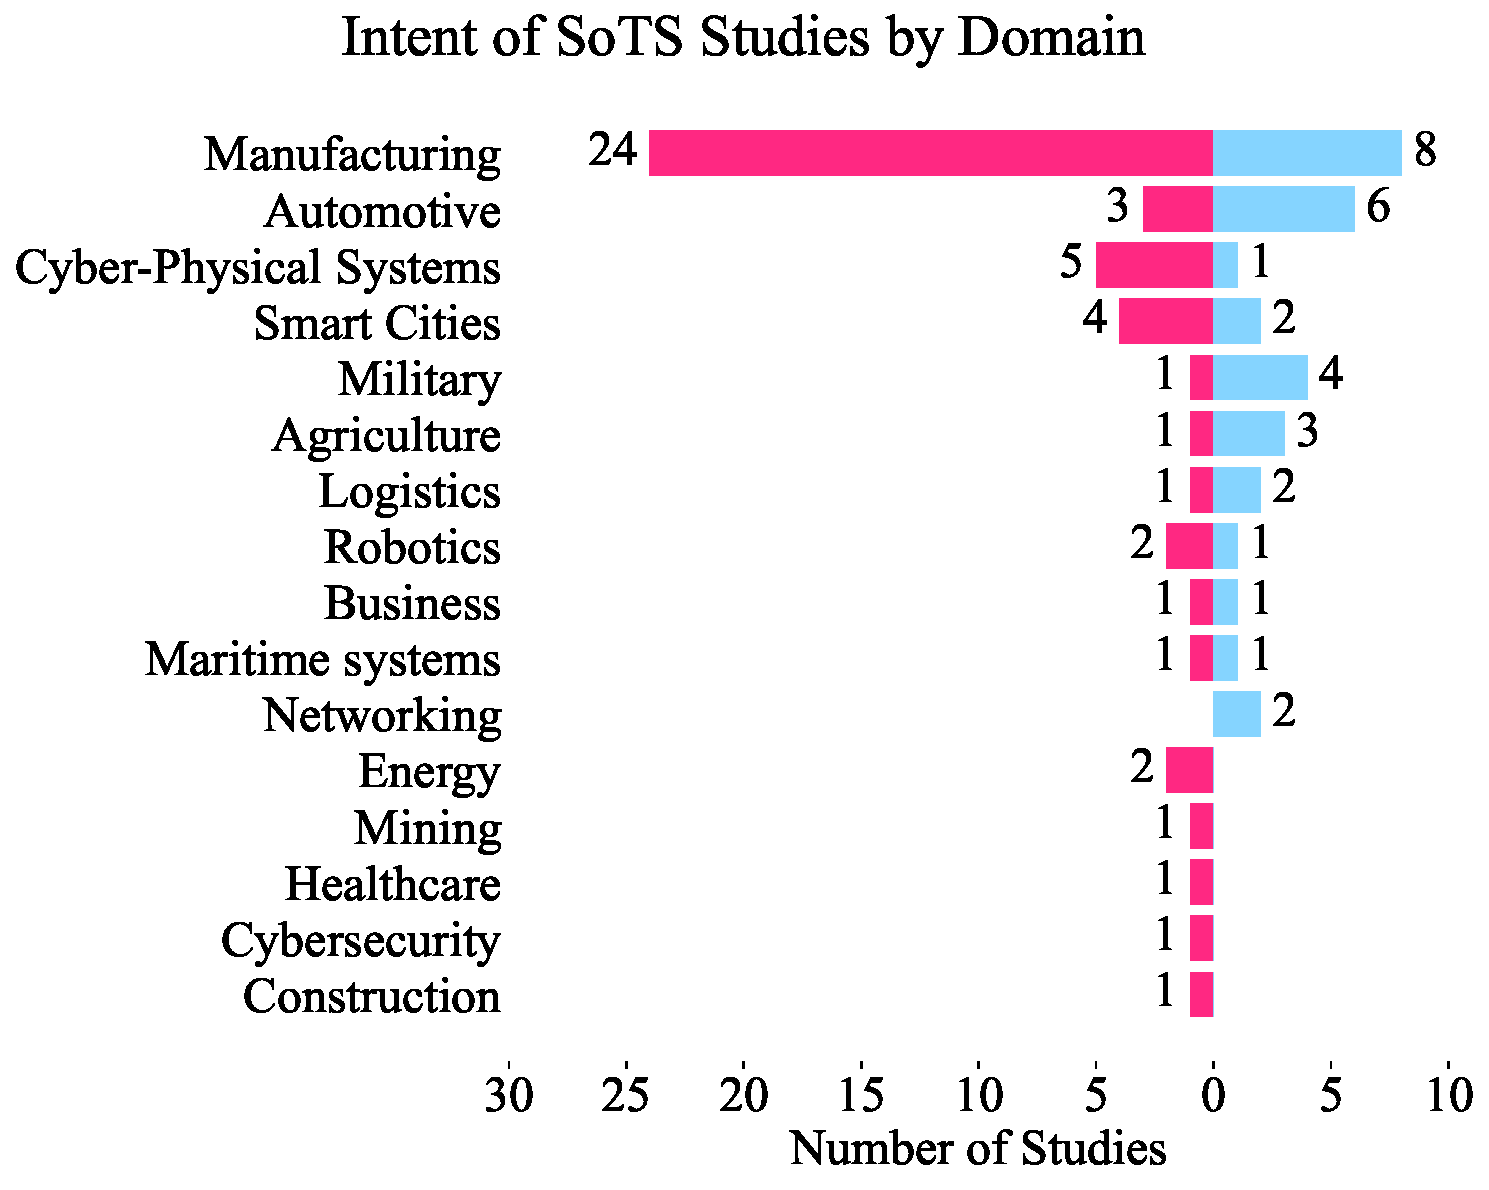
\includegraphics[width=0.65\linewidth]{figures/Literature Review/rq1/intentOfSoSDT.pdf}
    \caption{Intent of SoTS vs Domain\vspace{-1em}}
    \caption*{{\color[HTML]{FF2882}\ding{110}} Combining DTs into a SoS~~~{\color[HTML]{85d4ff}\ding{110}} Twinning a SoS }
    \label{fig:sos-dt-intent}
\end{figure}

Some domains appear exclusively under one approach. For example, networking appears only under twinning an SoS, where studies focus on holistic oversight of large-scale, dynamic communication infrastructures \cite{dobie2024network, priyanta2024is}. Energy, mining, healthcare, cybersecurity, and construction appear only under DT combination. 
Other domains, e.g., smart cities and logistics show both approaches.

As shown in \tabref{tab:domains-table}, the most frequently encountered domain is manufacturing (\xofyp{32}{80}), where SoTS are used to coordinate production lines and factory systems~\cite{gollner2022collaborative}. The automotive domain (\xofyp{9}{80}) applies SoTS for simulation-based testing, diagnostics, and control of vehicle subsystems~\cite{potteiger2023live}. In smart cities applications (\xofyp{6}{80}), SoTS support the modeling and integration of urban infrastructure~\cite{li2024comprehensive, human2023design}. The cyber-physical systems domain (\xofyp{6}{80}) focuses on managing real-time interaction between distributed physical processes and digital components~\cite{alam2017c2ps, stary2022privacy}.

Military, agriculture, logistics, and robotics applications appear in fewer than 6 studies each. The remaining 15\% span maritime, healthcare, construction, energy, and networking domains.

\begin{table*}[]
            \centering
            \footnotesize
            \caption{Application domains}
            \label{tab:domains-table}
            \begin{tabular}{@{}p{4cm}l p{8.5cm}@{}}
            \toprule
            \multicolumn{1}{c}{\textbf{Domain}} & 
            \multicolumn{1}{c}{\textbf{Frequency}} & 
            \multicolumn{1}{c}{\textbf{Studies}} \\ 
            \midrule
            Manufacturing & \maindatabar{32} & \cite{acharya2023twins,ashtaritalkhestani2019architecture,aziz2022empowering,bao2024digital,barden2022academic,bellavista2023requirements,binder2021utilizing,demir2023vertically-integrated,duan2023digital,ehemann2023digital,esterle2021digital,gill2022method,gollner2022collaborative,jirsa2024use,joseph2021aggregated,kruger2022towards,kutzke2021subsystem,larsen2024towards,lippi2023enabling,liu2020web-based,marah2023architecture,monsalve2021novel,novak2022digitalized,park2020digital,parri2019jarvis,redelinghuys2020six-layer,reiche2021digital,schluse2017experimentable,villalonga2021decision-making,vogel-heuser2021approach,zhang2021bi-level,zhang2022multi-scale} \\
Automotive & \maindatabar{9} & \cite{chen2018digital,dahmen2022modeling,heithoff2023challenges,malayjerdi2022combined,oquendo2019dealing,pillai2023digital,potteiger2023live,samak2023autodrive,vermesan2021internet} \\
Cyber-Physical Systems & \maindatabar{6} & \cite{alam2017c2ps,coupaye2023graph-based,li2022cognitive,mahoro2023articulating,parri2021framework,stary2022privacy} \\
Smart Cities & \maindatabar{6} & \cite{hofmeister2024cross-domain,hofmeister2024semantic,human2023design,li2024comprehensive,mavromatis2024umbrella,somma2023digital} \\
Military & \maindatabar{5} & \cite{folds2019digital,hatakeyama2018systems,lee2022simulation,lopez2023modeling,wang2024construction} \\
Agriculture & \maindatabar{4} & \cite{chavezbaliguat2023digital,howard2021greenhouse,pickering2023towards,saraeian2022digital} \\
Logistics & \maindatabar{3} & \cite{clark2021chapter,doubell2023digital,wagner2023using} \\
Robotics & \maindatabar{3} & \cite{gil2023modeling,gil2024integrating,savur2019hrc-sos} \\
Other & \maindatabar{12} & \cite{altamiranda2019system,becue2018cyberfactory,bertoni2022digital,dickopf2019holistic,dobie2024network,hatledal2020co-simulation,heininger2021capturing,jiang2022novel,kulkarni2019towards,maheshwari2022digital,priyanta2024is,wullink2024foundational} \\
\bottomrule
            \end{tabular}
            \end{table*}

\begin{conclusionframe}{RQ1: Why are DT and SoS combined}
SoTS are developed to support optimization, integration, validation, and maintainability in complex systems. Manufacturing is the most common application domain, followed by automotive and smart cities.
\end{conclusionframe}


\subsection{How are DT and SoS combined? (RQ2)}\label{results-rq2}

To understand how DT and SoS are combined, we analyze architectures (\secref{sec:architecture}) and types of constituent units (\secref{sec:constituents}) represented in SoTS.



\subsubsection{Architecture Configurations}\label{sec:architecture}

\begin{table*}[htp]
            \centering
            \scriptsize
            \caption{SoTS Type}
            \label{tab:sots-type-table}
            \begin{tabular}{@{}p{4cm}l p{8.5cm}@{}}
            \toprule
            \multicolumn{1}{c}{\textbf{SoTS}} & 
            \multicolumn{1}{c}{\textbf{Frequency}} & 
            \multicolumn{1}{c}{\textbf{Studies}} \\ 
            \midrule
            Acknowledged SoTS & \maindatabar{31} & \cite{altamiranda2019system,becue2018cyberfactory,bellavista2023requirements,bertoni2022digital,binder2021utilizing,coupaye2023graph-based,demir2023vertically-integrated,ehemann2023digital,folds2019digital,gill2022method,heininger2021capturing,heithoff2023challenges,human2023design,kruger2022towards,li2022cognitive,lippi2023enabling,lopez2023modeling,maheshwari2022digital,mahoro2023articulating,malayjerdi2022combined,monsalve2021novel,parri2019jarvis,pillai2023digital,potteiger2023live,priyanta2024is,redelinghuys2020six-layer,samak2023autodrive,saraeian2022digital,somma2023digital,wagner2023using,zhang2021bi-level} \\
Directed SoTS & \maindatabar{26} & \cite{alam2017c2ps,ashtaritalkhestani2019architecture,aziz2022empowering,chavezbaliguat2023digital,dickopf2019holistic,dobie2024network,doubell2023digital,duan2023digital,gil2024integrating,hatakeyama2018systems,hofmeister2024semantic,jiang2022novel,kulkarni2019towards,kutzke2021subsystem,larsen2024towards,lee2022simulation,li2024comprehensive,novak2022digitalized,park2020digital,parri2021framework,reiche2021digital,schluse2017experimentable,stary2022privacy,villalonga2021decision-making,wang2024construction,zhang2022multi-scale} \\
Collaborative SoTS & \maindatabar{19} & \cite{acharya2023twins,bao2024digital,barden2022academic,chen2018digital,dahmen2022modeling,gil2023modeling,gollner2022collaborative,hatledal2020co-simulation,hofmeister2024cross-domain,howard2021greenhouse,jirsa2024use,joseph2021aggregated,liu2020web-based,marah2023architecture,mavromatis2024umbrella,savur2019hrc-sos,vermesan2021internet,vogel-heuser2021approach,wullink2024foundational} \\
Virtual SoTS & \maindatabar{4} & \cite{clark2021chapter,esterle2021digital,oquendo2019dealing,pickering2023towards} \\
\bottomrule
            \end{tabular}
            \end{table*}

We applied our SoTS classification framework (\secref{sec:literature-review-classification}) to categorize the studies into distinct architectural types. These types reflect the degree of autonomy, goal alignment, and coordination mechanisms between constituent systems, with DTs acting as either orchestrators or peers. The distribution of studies across types is summarized in \tabref{tab:sots-type-table}.

The majority of studies followed an Acknowledged SoTS architecture (\xofyp{31}{80}). In these systems, a central DT facilitates coordination, but each constituent retains managerial independence and negotiates its own goals. For instance, \textcite{li2022cognitive} implements a cognitive twin that synthesizes simulations and provides recommendations to UAVs and USVs, which maintain control over their own missions. Similarly, in \textcite{monsalve2021novel}, a Digital Twin Master (DTM) oversees synchronization and data flow across grid simulations, while each local Digital Twin Client (DTC) retains its own model and operational logic.

A comparable number of studies implement a Directed SoTS  (\xofyp{26}{80}). These systems are governed by a central DT that imposes goals and orchestrates constituent behavior. In \textcite{reiche2021digital}, the Digital Twin of a System (DTS) aggregates and controls individual machine twins, using a dedicated interface (DTS2DT) to monitor operations, issue commands, and maintain an integrated simulation of the whole unit. Similarly, \textcite{li2024comprehensive} introduces an infrastructure DT that coordinates multiple civil subsystems under a unified scenario-based control structure.

Collaborative SoTS architectures were found in \xofyp{19}{80} studies. These systems are formed through voluntary cooperation among DTs, with no centralized controller enforcing goals. \textcite{vogel-heuser2021approach} presents a decentralized manufacturing system composed of DTs instantiated as autonomous agents. Each agent voluntarily engages in shared production tasks through local negotiation without relying on centralized orchestration. Additionally, \textcite{chen2018digital} describes a fleet of connected vehicles, each sharing its own behavioral DT to support collective driving decisions without central command. Coordination emerges dynamically through peer-to-peer risk assessments.

Some studies qualify as Virtual SoTS (\xofyp{4}{80}), where constituents join voluntarily, pursue independent goals, and coordinate dynamically without centralized control. \textcite{pickering2023towards} presents the MAS-H platform, where independent stakeholders operate autonomously while dynamically coordinating through an open DT and modular infrastructure. Goals such as labor efficiency or sustainability emerge from voluntary collaboration rather than centralized directives. Similarly, \textcite{esterle2021digital} explores a system of autonomous cyber-physical entities that self-integrate during encounters. Coordination arises through dynamic model exchange and adaptation using DTs, without pre-defined tasks.



\subsubsection{Constituent units}\label{sec:constituents}

\begin{table*}[]
            \centering
            \footnotesize
            \caption{Constituent units}
            \label{tab:constituent-units-table}
            \begin{tabular}{@{}p{4cm}l p{8.5cm}@{}}
            \toprule
            \multicolumn{1}{c}{\textbf{Constituent Unit}} & 
            \multicolumn{1}{c}{\textbf{Frequency}} & 
            \multicolumn{1}{c}{\textbf{Studies}} \\ 
            \midrule
            Physical Systems & \maindatabar{62} & \cite{acharya2023twins,altamiranda2019system,ashtaritalkhestani2019architecture,aziz2022empowering,bao2024digital,barden2022academic,becue2018cyberfactory,bellavista2023requirements,bertoni2022digital,binder2021utilizing,chavezbaliguat2023digital,chen2018digital,coupaye2023graph-based,dahmen2022modeling,demir2023vertically-integrated,dobie2024network,doubell2023digital,duan2023digital,ehemann2023digital,esterle2021digital,gil2023modeling,gill2022method,gollner2022collaborative,hatledal2020co-simulation,heininger2021capturing,heithoff2023challenges,hofmeister2024cross-domain,hofmeister2024semantic,howard2021greenhouse,human2023design,jiang2022novel,jirsa2024use,joseph2021aggregated,kruger2022towards,kutzke2021subsystem,larsen2024towards,lee2022simulation,li2022cognitive,li2024comprehensive,lippi2023enabling,liu2020web-based,lopez2023modeling,malayjerdi2022combined,monsalve2021novel,novak2022digitalized,oquendo2019dealing,park2020digital,pillai2023digital,potteiger2023live,redelinghuys2020six-layer,reiche2021digital,samak2023autodrive,saraeian2022digital,somma2023digital,vermesan2021internet,villalonga2021decision-making,vogel-heuser2021approach,wagner2023using,wang2024construction,wullink2024foundational,zhang2022multi-scale,zhang2021bi-level} \\
Cyber Physical Systems & \maindatabar{9} & \cite{alam2017c2ps,clark2021chapter,hatakeyama2018systems,mahoro2023articulating,marah2023architecture,mavromatis2024umbrella,priyanta2024is,schluse2017experimentable,stary2022privacy} \\
Cyber-Physical-Human Systems & \maindatabar{7} & \cite{dickopf2019holistic,folds2019digital,gil2024integrating,parri2021framework,parri2019jarvis,pickering2023towards,savur2019hrc-sos} \\
Enterprise Systems & \maindatabar{2} & \cite{kulkarni2019towards,maheshwari2022digital} \\
\bottomrule
            \end{tabular}
            \end{table*}

\tabref{tab:constituent-units-table} summarizes the types of constituent units in SoTS. Most studies (\xofyp{62}{80}) focus on physical systems, e.g., machines, vehicles, or industrial assets. These DTs support monitoring, control, and optimization at the asset or network level \cite{reiche2021digital, kruger2022towards}.
Cyber-Physical Systems (CPS) appear in (\xofyp{9}{80}) studies, where emphasis is placed on cross-domain interoperability and reusable architectures \cite{marah2023architecture, mahoro2023articulating}.
Cyber-Physical-Human Systems (CPHS) are considered in (\xofyp{7}{80}) studies, incorporating human interaction or oversight. Examples include human-robot collaboration and adaptive mission planning \cite{savur2019hrc-sos, folds2019digital}.
Only (\xofyp{2}{80}) studies address enterprise systems, modeling organizational entities, e.g., departments or administrative units as DTs \cite{kulkarni2019towards, maheshwari2022digital}.



\begin{conclusionframe}{RQ2: How DTs and SoS are combined}
Most SoTS adopt centralized architectures, with DTs coordinating physical systems via Acknowledged or Directed patterns. Decentralized forms like Collaborative and Virtual SoTS are less common. Constituents are primarily physical assets, with limited use of cyber-physical systems, cyber-physical-human systems, or enterprise-level twins.
\end{conclusionframe}



\subsection{What are the characteristics of DTs that are combined with SoS? (RQ3)}\label{results-rq3}

To find the characteristics of DTs used in SoTS we analyze their levels of autonomy (\secref{sec:level-of-autonomy}), the services they provide (\secref{sec:dt-services}), and the modeling and simulation techniques applied (\secref{sec:modeling-methods}).

\begin{figure*}[t]
    \centering
    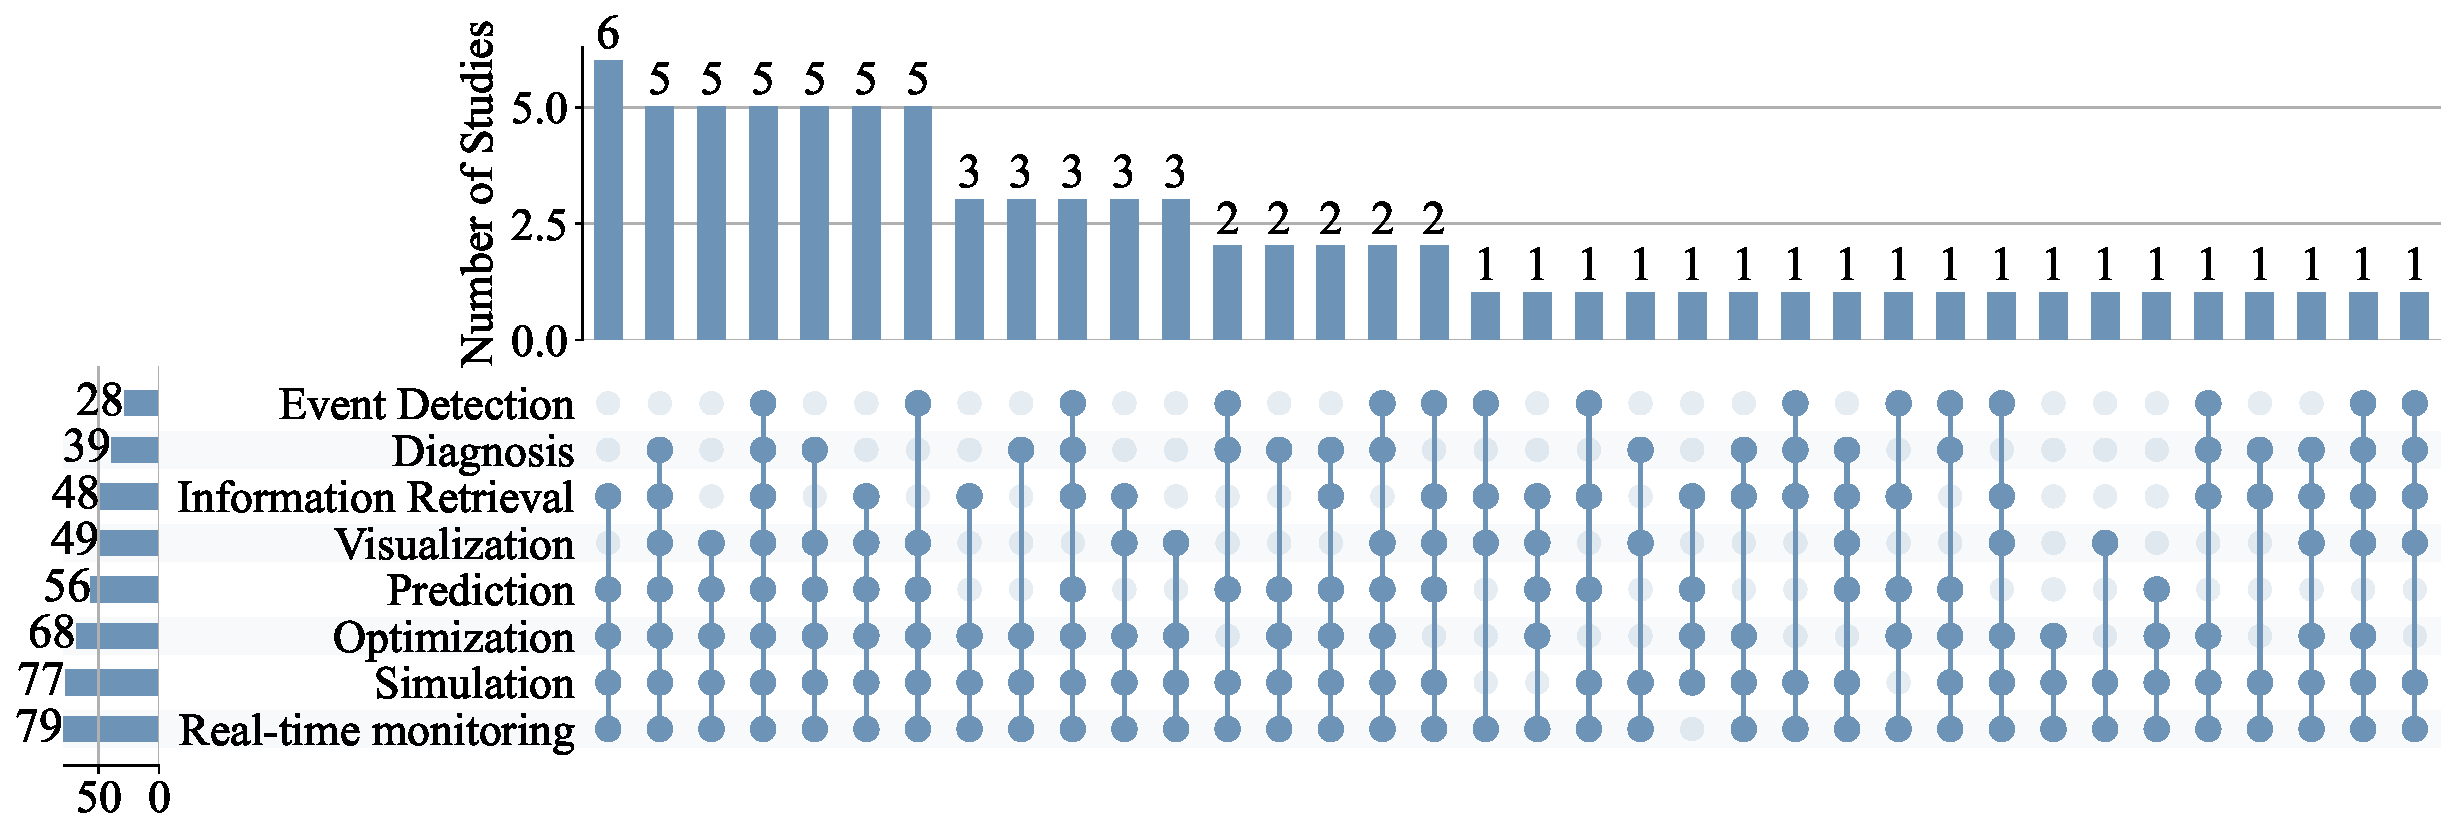
\includegraphics[width=\linewidth]{figures/Literature Review/rq3/dtServices.pdf}
    \caption{Combinations of DT services supported across reviewed SoTS studies}
    \label{fig:dt-services}
\end{figure*}


\subsubsection{Level of autonomy}\label{sec:level-of-autonomy}

\begin{table*}[]
            \centering
            \footnotesize
            \caption{Levels of autonomy}
            \label{tab:autonomy-table}
            \begin{tabular}{@{}p{4cm}l p{8.5cm}@{}}
            \toprule
            \multicolumn{1}{c}{\textbf{Autonomy}} & 
            \multicolumn{1}{c}{\textbf{Frequency}} & 
            \multicolumn{1}{c}{\textbf{Studies}} \\ 
            \midrule
            Digital Twin & \maindatabar{66} & \cite{acharya2023twins,alam2017c2ps,altamiranda2019system,ashtaritalkhestani2019architecture,aziz2022empowering,bao2024digital,barden2022academic,becue2018cyberfactory,bellavista2023requirements,binder2021utilizing,chen2018digital,clark2021chapter,coupaye2023graph-based,dahmen2022modeling,demir2023vertically-integrated,doubell2023digital,duan2023digital,ehemann2023digital,esterle2021digital,gil2023modeling,gill2022method,gollner2022collaborative,hatakeyama2018systems,hatledal2020co-simulation,heininger2021capturing,heithoff2023challenges,howard2021greenhouse,human2023design,jiang2022novel,jirsa2024use,joseph2021aggregated,kruger2022towards,kutzke2021subsystem,larsen2024towards,lee2022simulation,li2022cognitive,li2024comprehensive,lippi2023enabling,liu2020web-based,lopez2023modeling,maheshwari2022digital,mahoro2023articulating,malayjerdi2022combined,marah2023architecture,mavromatis2024umbrella,monsalve2021novel,novak2022digitalized,oquendo2019dealing,park2020digital,pillai2023digital,potteiger2023live,priyanta2024is,redelinghuys2020six-layer,reiche2021digital,samak2023autodrive,schluse2017experimentable,somma2023digital,stary2022privacy,vermesan2021internet,villalonga2021decision-making,vogel-heuser2021approach,wagner2023using,wang2024construction,wullink2024foundational,zhang2022multi-scale,zhang2021bi-level} \\
Digital Shadow & \maindatabar{6} & \cite{bertoni2022digital,chavezbaliguat2023digital,dobie2024network,hofmeister2024cross-domain,hofmeister2024semantic,saraeian2022digital} \\
Human-Supervised Digital Twin & \maindatabar{4} & \cite{folds2019digital,gil2024integrating,pickering2023towards,savur2019hrc-sos} \\
Human-Actuated Digital Twin & \maindatabar{3} & \cite{dickopf2019holistic,parri2021framework,parri2019jarvis} \\
Digital Model & \maindatabar{1} & \cite{kulkarni2019towards} \\
\bottomrule
            \end{tabular}
            \end{table*}

\tabref{tab:autonomy-table} summarizes the autonomy levels in SoTS DTs in accordance with the classifications of \textcite{kritzinger2018digital} and \textcite{david2024infonomics}. 
Most studies (\xofyp{66}{80}) implement fully autonomous DTs for independent monitoring, control, or decision-making.
Digital shadows, passive representations without autonomy, appear in (\xofyp{6}{80}) studies. \textcite{hofmeister2024semantic} use them as data layers for agents assessing environmental risks.
Human-supervised DTs appear in (\xofyp{4}{80}) studies and human-actuated DTs in (\xofyp{3}{80}), typically in safety-critical contexts. For example, \textcite{folds2019digital} use a supervised DT for mission adaptation in a cyber-physical-human system.
Only one study uses a digital model (\xofyp{1}{80}), representing static models, for enterprise-level planning rather than real-time operation \cite{kulkarni2019towards}.


\subsubsection{DT services}\label{sec:dt-services}

\begin{table*}[htp]
            \centering
            \scriptsize
            \caption{DT services supported}
            \label{tab:dt-services-table}
            \begin{tabular}{@{}p{4cm}l p{8.5cm}@{}}
            \toprule
            \multicolumn{1}{c}{\textbf{Service}} & 
            \multicolumn{1}{c}{\textbf{Frequency}} & 
            \multicolumn{1}{c}{\textbf{Studies}} \\ 
            \midrule
            Real-time monitoring & \maindatabar{79} & \cite{acharya2023twins,alam2017c2ps,altamiranda2019system,ashtaritalkhestani2019architecture,aziz2022empowering,bao2024digital,barden2022academic,becue2018cyberfactory,bellavista2023requirements,bertoni2022digital,binder2021utilizing,chavezbaliguat2023digital,chen2018digital,clark2021chapter,coupaye2023graph-based,dahmen2022modeling,demir2023vertically-integrated,dickopf2019holistic,dobie2024network,doubell2023digital,duan2023digital,ehemann2023digital,esterle2021digital,folds2019digital,gil2023modeling,gil2024integrating,gill2022method,gollner2022collaborative,hatakeyama2018systems,hatledal2020co-simulation,heininger2021capturing,heithoff2023challenges,hofmeister2024cross-domain,hofmeister2024semantic,howard2021greenhouse,human2023design,jiang2022novel,jirsa2024use,joseph2021aggregated,kruger2022towards,kutzke2021subsystem,larsen2024towards,lee2022simulation,li2022cognitive,li2024comprehensive,lippi2023enabling,liu2020web-based,lopez2023modeling,maheshwari2022digital,mahoro2023articulating,malayjerdi2022combined,marah2023architecture,mavromatis2024umbrella,monsalve2021novel,novak2022digitalized,oquendo2019dealing,park2020digital,parri2021framework,parri2019jarvis,pickering2023towards,pillai2023digital,potteiger2023live,priyanta2024is,redelinghuys2020six-layer,reiche2021digital,samak2023autodrive,saraeian2022digital,savur2019hrc-sos,schluse2017experimentable,somma2023digital,stary2022privacy,vermesan2021internet,villalonga2021decision-making,vogel-heuser2021approach,wagner2023using,wang2024construction,wullink2024foundational,zhang2022multi-scale,zhang2021bi-level} \\
Simulation & \maindatabar{77} & \cite{acharya2023twins,alam2017c2ps,altamiranda2019system,ashtaritalkhestani2019architecture,bao2024digital,barden2022academic,becue2018cyberfactory,bellavista2023requirements,bertoni2022digital,binder2021utilizing,chen2018digital,clark2021chapter,coupaye2023graph-based,dahmen2022modeling,demir2023vertically-integrated,dickopf2019holistic,dobie2024network,doubell2023digital,duan2023digital,ehemann2023digital,esterle2021digital,folds2019digital,gil2023modeling,gil2024integrating,gill2022method,gollner2022collaborative,hatakeyama2018systems,hatledal2020co-simulation,heininger2021capturing,heithoff2023challenges,hofmeister2024cross-domain,hofmeister2024semantic,howard2021greenhouse,human2023design,jiang2022novel,jirsa2024use,joseph2021aggregated,kruger2022towards,kulkarni2019towards,kutzke2021subsystem,larsen2024towards,lee2022simulation,li2022cognitive,li2024comprehensive,lippi2023enabling,liu2020web-based,lopez2023modeling,maheshwari2022digital,mahoro2023articulating,malayjerdi2022combined,marah2023architecture,mavromatis2024umbrella,monsalve2021novel,novak2022digitalized,oquendo2019dealing,park2020digital,parri2021framework,parri2019jarvis,pickering2023towards,potteiger2023live,priyanta2024is,redelinghuys2020six-layer,reiche2021digital,samak2023autodrive,saraeian2022digital,savur2019hrc-sos,schluse2017experimentable,somma2023digital,stary2022privacy,vermesan2021internet,villalonga2021decision-making,vogel-heuser2021approach,wagner2023using,wang2024construction,wullink2024foundational,zhang2022multi-scale,zhang2021bi-level} \\
Optimization & \maindatabar{68} & \cite{acharya2023twins,alam2017c2ps,altamiranda2019system,ashtaritalkhestani2019architecture,bao2024digital,barden2022academic,becue2018cyberfactory,bellavista2023requirements,bertoni2022digital,binder2021utilizing,chavezbaliguat2023digital,chen2018digital,clark2021chapter,coupaye2023graph-based,demir2023vertically-integrated,dickopf2019holistic,dobie2024network,doubell2023digital,duan2023digital,ehemann2023digital,esterle2021digital,folds2019digital,gil2023modeling,gil2024integrating,gill2022method,hatakeyama2018systems,hatledal2020co-simulation,heininger2021capturing,heithoff2023challenges,howard2021greenhouse,jiang2022novel,jirsa2024use,joseph2021aggregated,kruger2022towards,kulkarni2019towards,kutzke2021subsystem,larsen2024towards,lee2022simulation,li2022cognitive,li2024comprehensive,lippi2023enabling,liu2020web-based,maheshwari2022digital,mahoro2023articulating,malayjerdi2022combined,marah2023architecture,mavromatis2024umbrella,monsalve2021novel,novak2022digitalized,oquendo2019dealing,park2020digital,pickering2023towards,pillai2023digital,potteiger2023live,priyanta2024is,redelinghuys2020six-layer,samak2023autodrive,saraeian2022digital,schluse2017experimentable,somma2023digital,vermesan2021internet,villalonga2021decision-making,vogel-heuser2021approach,wagner2023using,wang2024construction,wullink2024foundational,zhang2022multi-scale,zhang2021bi-level} \\
Prediction & \maindatabar{56} & \cite{acharya2023twins,alam2017c2ps,altamiranda2019system,ashtaritalkhestani2019architecture,bao2024digital,barden2022academic,becue2018cyberfactory,bellavista2023requirements,bertoni2022digital,chavezbaliguat2023digital,chen2018digital,clark2021chapter,coupaye2023graph-based,dahmen2022modeling,demir2023vertically-integrated,dickopf2019holistic,dobie2024network,doubell2023digital,duan2023digital,ehemann2023digital,esterle2021digital,folds2019digital,gollner2022collaborative,hatakeyama2018systems,hatledal2020co-simulation,heininger2021capturing,hofmeister2024cross-domain,hofmeister2024semantic,howard2021greenhouse,jiang2022novel,joseph2021aggregated,kulkarni2019towards,kutzke2021subsystem,larsen2024towards,li2022cognitive,li2024comprehensive,lippi2023enabling,maheshwari2022digital,mahoro2023articulating,marah2023architecture,novak2022digitalized,oquendo2019dealing,park2020digital,parri2021framework,parri2019jarvis,pickering2023towards,pillai2023digital,priyanta2024is,samak2023autodrive,saraeian2022digital,somma2023digital,villalonga2021decision-making,wagner2023using,wang2024construction,wullink2024foundational,zhang2022multi-scale} \\
Visualization & \maindatabar{49} & \cite{acharya2023twins,alam2017c2ps,altamiranda2019system,ashtaritalkhestani2019architecture,aziz2022empowering,bao2024digital,barden2022academic,bertoni2022digital,chavezbaliguat2023digital,chen2018digital,coupaye2023graph-based,dahmen2022modeling,demir2023vertically-integrated,dickopf2019holistic,dobie2024network,doubell2023digital,duan2023digital,ehemann2023digital,esterle2021digital,folds2019digital,hatledal2020co-simulation,hofmeister2024cross-domain,hofmeister2024semantic,howard2021greenhouse,jirsa2024use,joseph2021aggregated,kruger2022towards,larsen2024towards,lee2022simulation,li2024comprehensive,liu2020web-based,lopez2023modeling,maheshwari2022digital,mahoro2023articulating,malayjerdi2022combined,marah2023architecture,mavromatis2024umbrella,pickering2023towards,potteiger2023live,priyanta2024is,redelinghuys2020six-layer,samak2023autodrive,savur2019hrc-sos,schluse2017experimentable,somma2023digital,stary2022privacy,villalonga2021decision-making,wang2024construction,wullink2024foundational} \\
Information Retrieval & \maindatabar{48} & \cite{acharya2023twins,alam2017c2ps,altamiranda2019system,ashtaritalkhestani2019architecture,aziz2022empowering,becue2018cyberfactory,bellavista2023requirements,binder2021utilizing,chavezbaliguat2023digital,clark2021chapter,coupaye2023graph-based,dahmen2022modeling,demir2023vertically-integrated,dickopf2019holistic,dobie2024network,doubell2023digital,ehemann2023digital,gil2024integrating,gollner2022collaborative,hatakeyama2018systems,heininger2021capturing,heithoff2023challenges,hofmeister2024cross-domain,hofmeister2024semantic,howard2021greenhouse,human2023design,jiang2022novel,jirsa2024use,kruger2022towards,kulkarni2019towards,kutzke2021subsystem,larsen2024towards,lee2022simulation,li2022cognitive,li2024comprehensive,lippi2023enabling,liu2020web-based,maheshwari2022digital,mavromatis2024umbrella,novak2022digitalized,oquendo2019dealing,pillai2023digital,redelinghuys2020six-layer,reiche2021digital,somma2023digital,stary2022privacy,vogel-heuser2021approach,zhang2021bi-level} \\
Diagnosis & \maindatabar{39} & \cite{acharya2023twins,alam2017c2ps,altamiranda2019system,ashtaritalkhestani2019architecture,bao2024digital,becue2018cyberfactory,bellavista2023requirements,clark2021chapter,coupaye2023graph-based,dahmen2022modeling,dickopf2019holistic,dobie2024network,doubell2023digital,duan2023digital,esterle2021digital,folds2019digital,gil2023modeling,gill2022method,heithoff2023challenges,howard2021greenhouse,human2023design,jiang2022novel,kruger2022towards,li2024comprehensive,lippi2023enabling,liu2020web-based,lopez2023modeling,marah2023architecture,monsalve2021novel,park2020digital,parri2021framework,parri2019jarvis,reiche2021digital,saraeian2022digital,stary2022privacy,villalonga2021decision-making,wullink2024foundational,zhang2022multi-scale,zhang2021bi-level} \\
Event Detection & \maindatabar{28} & \cite{alam2017c2ps,aziz2022empowering,bao2024digital,becue2018cyberfactory,chen2018digital,clark2021chapter,coupaye2023graph-based,dobie2024network,doubell2023digital,gollner2022collaborative,hofmeister2024cross-domain,hofmeister2024semantic,human2023design,joseph2021aggregated,li2024comprehensive,lippi2023enabling,liu2020web-based,mahoro2023articulating,mavromatis2024umbrella,park2020digital,parri2021framework,parri2019jarvis,pickering2023towards,pillai2023digital,stary2022privacy,villalonga2021decision-making,wang2024construction,zhang2021bi-level} \\
\bottomrule
            \end{tabular}
            \end{table*}

\tabref{tab:dt-services-table} summarizes the services provided by DTs in SoTS configurations. As shown in \figref{fig:dt-services}, most studies combine multiple services rather than using them in isolation.

The most widely used services are real-time monitoring (\xofyp{79}{80}), simulation (\xofyp{77}{80}), and optimization (\xofyp{68}{80}). Prediction (\xofyp{56}{80}), visualization (\xofyp{49}{80}), and information retrieval (\xofyp{48}{80}) are also frequently integrated.

The most common service combination, observed in \xofyp{6}{80} studies, includes real-time monitoring, simulation, optimization, prediction, and information retrieval, supporting both continuous system supervision and proactive planning. Other studies incorporate varied combinations, typically coupling the core services (monitoring, simulation, optimization, and prediction) with additional functionalities, e.g., visualization, information retrieval, diagnosis, and event detection.



\subsubsection{Modeling and simulation formalisms and techniques}\label{sec:modeling-methods}

\begin{table*}[]
\centering
\setlength{\tabcolsep}{1em}
\caption{Modeling and simulation formalisms}
\label{tab:modeling-methods-structured-table}
\scriptsize
\begin{tabular}{@{}p{5cm} l p{7.5cm}@{}}
\toprule
\textbf{Category} & \textbf{Frequency} & \textbf{Studies} \\
\midrule
\textbf{Architectural and Structural} & \textbf{\maindatabar{31}} & \\
\;\;\corner{} Systems Modeling Language (SysML) & \subdatabar{13} & \cite{ashtaritalkhestani2019architecture,dahmen2022modeling,dickopf2019holistic,gollner2022collaborative,jiang2022novel,kutzke2021subsystem,lopez2023modeling,parri2019jarvis,parri2021framework,pickering2023towards,schluse2017experimentable,wagner2023using,zhang2022multi-scale} \\
\;\;\corner{} Unified Modeling Language (UML) & \subdatabar{12} & \cite{dahmen2022modeling,duan2023digital,gil2024integrating,gill2022method,gollner2022collaborative,heithoff2023challenges,hofmeister2024semantic,jiang2022novel,lee2022simulation,parri2019jarvis,parri2021framework,vogel-heuser2021approach} \\
\;\;\corner{} Business Process Modeling (BPM) & \subdatabar{3} & \cite{binder2021utilizing,kulkarni2019towards,vogel-heuser2021approach} \\
\;\;\corner{} Building Information Modeling (BIM) & \subdatabar{3} & \cite{coupaye2023graph-based,doubell2023digital,larsen2024towards} \\
\;\;\corner{} Subject-Oriented Modeling (S-BPM) & \subdatabar{2} & \cite{heininger2021capturing,stary2022privacy} \\
\;\;\corner{} State Models & \subdatabar{2} & \cite{kruger2022towards,reiche2021digital} \\
\;\;\corner{} \textit{Other} & \subdatabar{8} & \cite{binder2021utilizing,dahmen2022modeling,dobie2024network,gil2024integrating,gollner2022collaborative,kulkarni2019towards,villalonga2021decision-making,wagner2023using} \\
\textbf{Spatial and Visual Modeling} & \textbf{\maindatabar{24}} & \\
\;\;\corner{} Computer-Aided Design (CAD) & \subdatabar{12} & \cite{ashtaritalkhestani2019architecture,becue2018cyberfactory,coupaye2023graph-based,duan2023digital,ehemann2023digital,jiang2022novel,joseph2021aggregated,liu2020web-based,novak2022digitalized,park2020digital,reiche2021digital,zhang2021bi-level} \\
\;\;\corner{} 3D Modeling & \subdatabar{10} & \cite{bao2024digital,chavezbaliguat2023digital,ehemann2023digital,hatledal2020co-simulation,malayjerdi2022combined,mavromatis2024umbrella,priyanta2024is,samak2023autodrive,somma2023digital,vermesan2021internet} \\
\;\;\corner{} Geometric Models & \subdatabar{2} & \cite{duan2023digital,ehemann2023digital} \\
\;\;\corner{} Parametric Models & \subdatabar{2} & \cite{li2024comprehensive,wagner2023using} \\
\;\;\corner{} \textit{Other} & \subdatabar{6} & \cite{becue2018cyberfactory,chavezbaliguat2023digital,coupaye2023graph-based,demir2023vertically-integrated,ehemann2023digital,priyanta2024is} \\
\textbf{Mathematical and Statistical} & \textbf{\maindatabar{23}} & \\
\;\;\corner{} Bayesian Networks (BN) & \subdatabar{5} & \cite{alam2017c2ps,kutzke2021subsystem,lippi2023enabling,maheshwari2022digital,vogel-heuser2021approach} \\
\;\;\corner{} General Mathematical Models & \subdatabar{5} & \cite{hatledal2020co-simulation,howard2021greenhouse,jiang2022novel,kruger2022towards,maheshwari2022digital} \\
\;\;\corner{} Fuzzy Logic & \subdatabar{2} & \cite{alam2017c2ps,altamiranda2019system} \\
\;\;\corner{} Model Reference Adaptive Control (MRAC) & \subdatabar{2} & \cite{clark2021chapter,kulkarni2019towards} \\
\;\;\corner{} \textit{Other} & \subdatabar{18} & \cite{altamiranda2019system,barden2022academic,bertoni2022digital,chavezbaliguat2023digital,dobie2024network,esterle2021digital,folds2019digital,gil2023modeling,gill2022method,heininger2021capturing,howard2021greenhouse,jiang2022novel,kulkarni2019towards,lippi2023enabling,maheshwari2022digital,pillai2023digital,saraeian2022digital,vogel-heuser2021approach} \\
\textbf{Ontological and Knowledge Representation} & \textbf{\maindatabar{19}} & \\
\;\;\corner{} Web Ontology Language (OWL) & \subdatabar{7} & \cite{ashtaritalkhestani2019architecture,bao2024digital,gil2023modeling,hofmeister2024semantic,jiang2022novel,li2024comprehensive,liu2020web-based} \\
\;\;\corner{} AutomationML & \subdatabar{5} & \cite{ashtaritalkhestani2019architecture,gil2023modeling,gollner2022collaborative,liu2020web-based,novak2022digitalized} \\
\;\;\corner{} Resource Description Framework (RDF) & \subdatabar{3} & \cite{coupaye2023graph-based,hofmeister2024semantic,li2024comprehensive} \\
\;\;\corner{} Property Graphs (PGs) & \subdatabar{2} & \cite{coupaye2023graph-based,mahoro2023articulating} \\
\;\;\corner{} Information Model & \subdatabar{2} & \cite{hatledal2020co-simulation,reiche2021digital} \\
\;\;\corner{} \textit{Other} & \subdatabar{10} & \cite{coupaye2023graph-based,demir2023vertically-integrated,gil2023modeling,hofmeister2024cross-domain,hofmeister2024semantic,li2022cognitive,li2024comprehensive,monsalve2021novel,park2020digital,pickering2023towards} \\
\textbf{Formal and State Based Methods} & \textbf{\maindatabar{14}} & \\
\;\;\corner{} Finite State Machines (FSM) & \subdatabar{5} & \cite{alam2017c2ps,dahmen2022modeling,liu2020web-based,savur2019hrc-sos,vogel-heuser2021approach} \\
\;\;\corner{} Fault Tree Analysis (FTA) & \subdatabar{3} & \cite{parri2019jarvis,parri2021framework,saraeian2022digital} \\
\;\;\corner{} \textit{Other} & \subdatabar{7} & \cite{chen2018digital,hatledal2020co-simulation,heininger2021capturing,heithoff2023challenges,larsen2024towards,oquendo2019dealing,parri2019jarvis} \\
\textbf{AI and Machine Learning} & \textbf{\maindatabar{13}} & \\
\;\;\corner{} Machine Learning & \subdatabar{4} & \cite{dobie2024network,esterle2021digital,folds2019digital,jiang2022novel} \\
\;\;\corner{} Reinforcement Learning (RL) & \subdatabar{2} & \cite{clark2021chapter,kulkarni2019towards} \\
\;\;\corner{} Genetic Algorithms (GA) & \subdatabar{2} & \cite{kutzke2021subsystem,park2020digital} \\
\;\;\corner{} \textit{Other} & \subdatabar{5} & \cite{altamiranda2019system,bao2024digital,chen2018digital,saraeian2022digital,villalonga2021decision-making} \\
\textbf{Continuous Simulation} & \textbf{\maindatabar{12}} & \\
\;\;\corner{} System Dynamics Models (SDM) & \subdatabar{4} & \cite{folds2019digital,gill2022method,kulkarni2019towards,pickering2023towards} \\
\;\;\corner{} Kinematic Models & \subdatabar{3} & \cite{duan2023digital,gil2023modeling,schluse2017experimentable} \\
\;\;\corner{} General Physics Models & \subdatabar{2} & \cite{demir2023vertically-integrated,hatakeyama2018systems} \\
\;\;\corner{} Finite Element Method (FEM) & \subdatabar{2} & \cite{demir2023vertically-integrated,li2024comprehensive} \\
\;\;\corner{} \textit{Other} & \subdatabar{4} & \cite{altamiranda2019system,demir2023vertically-integrated,gil2023modeling,monsalve2021novel} \\
\textbf{Agent-Based Simulation} & \textbf{\maindatabar{10}} & \\
\;\;\corner{} Multi Agent System (MAS) & \subdatabar{9} & \cite{clark2021chapter,heininger2021capturing,howard2021greenhouse,jirsa2024use,liu2020web-based,marah2023architecture,samak2023autodrive,vogel-heuser2021approach,zhang2021bi-level} \\
\;\;\corner{} Agent Based Modeling (ABM) & \subdatabar{2} & \cite{barden2022academic,clark2021chapter} \\
\;\;\corner{} \textit{Other} & \subdatabar{1} & \cite{marah2023architecture} \\
\textbf{Discrete-Event Simulation} & \textbf{\maindatabar{8}} & \\
\;\;\corner{} Discrete Event Simulation (DES) & \subdatabar{4} & \cite{bertoni2022digital,clark2021chapter,demir2023vertically-integrated,villalonga2021decision-making} \\
\;\;\corner{} Discrete Event System Specification (DEVS) & \subdatabar{2} & \cite{lee2022simulation,oquendo2019dealing} \\
\;\;\corner{} \textit{Other} & \subdatabar{3} & \cite{lee2022simulation,wang2024construction,zhang2022multi-scale} \\
\bottomrule
\end{tabular}
\end{table*}

\tabref{tab:modeling-methods-structured-table} summarizes the modeling and simulation formalisms used in SoTS studies. Architectural and structural methods are most common (\xofyp{31}{80}), with UML (\xofyp{12}{80}) and SysML (\xofyp{11}{80}) for system specification. Spatial and visual models appear in (\xofyp{24}{80}) studies, including CAD (\xofyp{12}{80}) and 3D modeling (\xofyp{10}{80}) for physical layout and geometry. Mathematical and statistical models (\xofyp{23}{80}) support dynamics and uncertainty, often using Bayesian networks (BN) or general equations.
Ontological methods (\xofyp{19}{80}) address semantic integration via Web Ontology Language (OWL) and AutomationML. Formal methods (\xofyp{14}{80}) use Finite State Machines (FSM) and Fault Tree Analysis (FTA) for verification. AI/ML (\xofyp{13}{80}) enable adaptive learning. Continuous simulation methods (\xofyp{12}{80}) and agent-based simulations (\xofyp{10}{80}) model physical dynamics and interactions. Discrete-event simulation methods (\xofyp{8}{80}) are used for workflow and performance analysis.

\add{At this point, we recall the previously discussed inherent limitation of the study (\secref{sec:threats}) that the technical and technological choices we observe are not necessarily universal best practices to implement SoTS, they are mere tendencies in an emerging field. With the maturation of the field, better technical and technological choices may emerge.}

\begin{conclusionframe}{RQ3: Characteristics of DTs in SoTS}
Most SoTS use fully autonomous DTs that provide monitoring, simulation, prediction, and optimization services. Modeling approaches vary, with architectural, visual, and mathematical formalisms being the most frequently used.
\end{conclusionframe}


\subsection{What are the characteristics of SoS that are combined with DTs? (RQ4)}\label{results-rq4}

To identify the characteristics of SoS used in SoTS, we analyze their supported SoS dimensions (\secref{sec:dimensions}) and the forms of emergent behavior they exhibit (\secref{sec:emergence-type}).

\subsubsection{Dimensions of SoS}\label{sec:dimensions}

\begin{figure*}[htb]
    \centering
     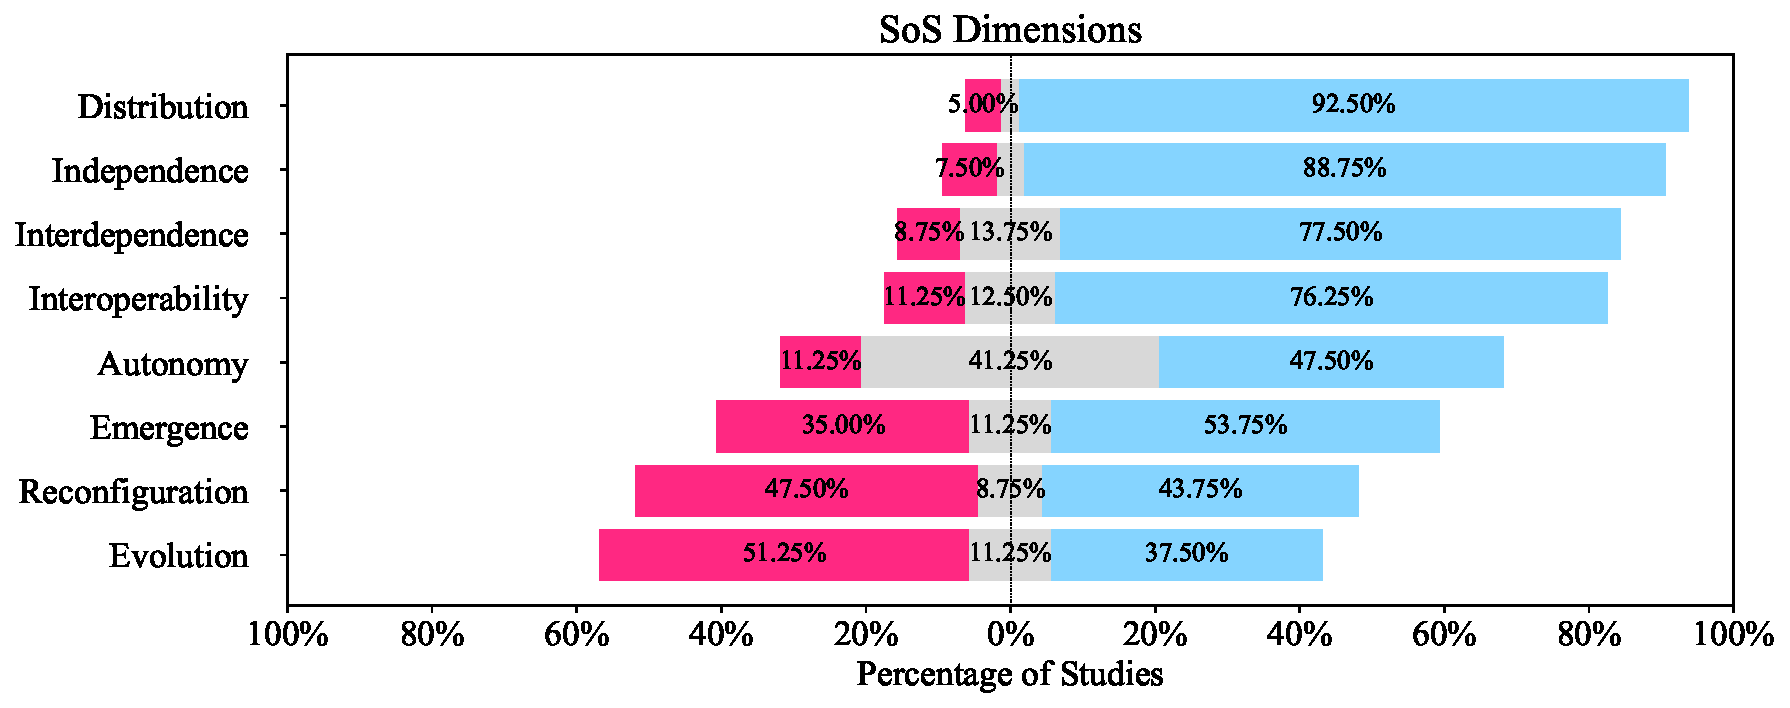
\includegraphics[width=\linewidth]{figures/Literature Review/rq4/sosDimensions.pdf}
    \caption{SoS dimensions: 
     {\color[HTML]{ff2882}\ding{108}} No,  
     {\color[HTML]{d8d8d8}\ding{108}} Partial, 
     {\color[HTML]{85d4ff}\ding{108}} Yes
    } 
    \label{fig:sos-dim}
\end{figure*}

\figref{fig:sos-dim} shows the SoS dimensions addressed in the studies. We follow the coding of SoS dimensions of \textcite{nielsen2015systems} and mark each SoS property either as explicitly present, partially evident, or absent. The system in the primary study is still considered a SoS as long as the primary study positions it as such.

The most frequently reported and investigated dimensions are distribution (\xofyp{74}{80}) and independence (\xofy{71}{80}). Interdependence (\xofyp{62}{80}) and interoperability (\xofyp{61}{80}) appear frequently as well, highlighting the perceived importance of coordination and information exchange in SoTS. Autonomy (\xofyp{38}{80} present and \xofyp{33}{80} partially present) and emergence (\xofyp{43}{80}) are less frequently addressed, with a substantial number of studies only partially addressing these properties. Reconfiguration (\xofyp{35}{80}) and evolution (\xofyp{30}{80}) are the least acknowledged SoS dimensions.


\subsubsection{Emergence type}\label{sec:emergence-type}

\tabref{tab:emergence-type-table} shows the types of emergent behavior reported in the studies. Weak emergence is most common (\xofyp{30}{80}). It involves behaviors that appear in system-level simulations but not in isolated components. \textcite{malayjerdi2022combined} demonstrate this through vehicle safety testing in software-in-the-loop setups. 
Simple emergence appears in (\xofyp{16}{80}) studies. It involves predictable interactions, e.g., in \textcite{zhang2022multi-scale}’s DT framework for shop floor coordination. 
Strong emergence is rare (\xofyp{6}{80}). It captures behaviors not predictable from subsystems. Examples include SoS simulations in mining \cite{bertoni2022digital} and automotive systems \cite{dahmen2022modeling}. (\xofyp{28}{80}) studies do not address emergent behaviors at all.



\begin{conclusionframe}{RQ4: Characteristics of SoS in SoTS}
SoTS support architectural SoS dimensions (distribution, independence, interdependence, and interoperability) but rarely address dynamical aspects (emergence, reconfiguration, and evolution). Emergent behavior is addressed in two thirds of the studies, most often as weak emergence, and many studies do not consider emergence at all.
\end{conclusionframe}

\begin{table*}[]
            \centering
            \footnotesize
            \caption{Emergence type}
            \label{tab:emergence-type-table}
            \begin{tabular}{@{}p{4cm}l p{8.5cm}@{}}
            \toprule
            \multicolumn{1}{c}{\textbf{Emergence}} & 
            \multicolumn{1}{c}{\textbf{Frequency}} & 
            \multicolumn{1}{c}{\textbf{Studies}} \\ 
            \midrule
            Not Addressed & \maindatabar{28} & \cite{acharya2023twins,ashtaritalkhestani2019architecture,aziz2022empowering,becue2018cyberfactory,binder2021utilizing,chavezbaliguat2023digital,doubell2023digital,duan2023digital,gil2023modeling,gollner2022collaborative,hatakeyama2018systems,hatledal2020co-simulation,heithoff2023challenges,hofmeister2024semantic,howard2021greenhouse,human2023design,kruger2022towards,kutzke2021subsystem,li2024comprehensive,liu2020web-based,mahoro2023articulating,marah2023architecture,monsalve2021novel,redelinghuys2020six-layer,reiche2021digital,villalonga2021decision-making,vogel-heuser2021approach,zhang2021bi-level} \\
Simple & \maindatabar{16} & \cite{gil2024integrating,lee2022simulation,li2022cognitive,lopez2023modeling,maheshwari2022digital,novak2022digitalized,park2020digital,parri2021framework,pillai2023digital,potteiger2023live,priyanta2024is,samak2023autodrive,somma2023digital,vermesan2021internet,wagner2023using,zhang2022multi-scale} \\
Weak & \maindatabar{30} & \cite{alam2017c2ps,altamiranda2019system,bao2024digital,barden2022academic,bellavista2023requirements,bertoni2022digital,chen2018digital,clark2021chapter,coupaye2023graph-based,demir2023vertically-integrated,dickopf2019holistic,dobie2024network,ehemann2023digital,esterle2021digital,gill2022method,heininger2021capturing,hofmeister2024cross-domain,larsen2024towards,lippi2023enabling,malayjerdi2022combined,mavromatis2024umbrella,oquendo2019dealing,parri2019jarvis,pickering2023towards,saraeian2022digital,savur2019hrc-sos,schluse2017experimentable,stary2022privacy,wang2024construction,wullink2024foundational} \\
Strong & \maindatabar{6} & \cite{dahmen2022modeling,folds2019digital,jiang2022novel,jirsa2024use,joseph2021aggregated,kulkarni2019towards} \\
\bottomrule
            \end{tabular}
            \end{table*}



\subsection{How are non-functional properties addressed in systems that combine SoS and DT? (RQ5)}\label{results-rq5}

To understand how non-functional properties---specifically, reliability (i.e., continuity of correct service~\cite{avizienis2004basic}) and security---are handled in SoTS, we analyze whether such considerations are addressed in the system requirements, architecture, or implementation, and whether they are evaluated or validated.

\begin{table*}[htp]
            \centering
            \footnotesize
            \caption{Reliability}
            \label{tab:reliability-table}
            \begin{tabular}{@{}p{4cm}l p{8.5cm}@{}}
            \toprule
            \multicolumn{1}{c}{\textbf{Context}} & 
            \multicolumn{1}{c}{\textbf{Frequency}} & 
            \multicolumn{1}{c}{\textbf{Studies}} \\ 
            \midrule
            Not Addressed & \maindatabar{26} & \cite{bao2024digital,bertoni2022digital,binder2021utilizing,clark2021chapter,coupaye2023graph-based,dahmen2022modeling,demir2023vertically-integrated,dickopf2019holistic,ehemann2023digital,gil2023modeling,gil2024integrating,gollner2022collaborative,hatakeyama2018systems,jiang2022novel,li2022cognitive,li2024comprehensive,maheshwari2022digital,mahoro2023articulating,reiche2021digital,samak2023autodrive,schluse2017experimentable,somma2023digital,stary2022privacy,wagner2023using,wang2024construction,zhang2022multi-scale} \\
Mentioned & \maindatabar{8} & \cite{barden2022academic,becue2018cyberfactory,heininger2021capturing,jirsa2024use,lee2022simulation,marah2023architecture,pickering2023towards,wullink2024foundational} \\
Architecturally Addressed & \maindatabar{41} & \cite{acharya2023twins,alam2017c2ps,altamiranda2019system,ashtaritalkhestani2019architecture,aziz2022empowering,bellavista2023requirements,chavezbaliguat2023digital,chen2018digital,dobie2024network,doubell2023digital,duan2023digital,esterle2021digital,folds2019digital,gill2022method,hatledal2020co-simulation,heithoff2023challenges,hofmeister2024cross-domain,hofmeister2024semantic,howard2021greenhouse,human2023design,joseph2021aggregated,kruger2022towards,kulkarni2019towards,larsen2024towards,lippi2023enabling,liu2020web-based,lopez2023modeling,mavromatis2024umbrella,monsalve2021novel,novak2022digitalized,parri2021framework,parri2019jarvis,pillai2023digital,potteiger2023live,priyanta2024is,redelinghuys2020six-layer,savur2019hrc-sos,vermesan2021internet,villalonga2021decision-making,vogel-heuser2021approach,zhang2021bi-level} \\
Explicitly Modeled & \maindatabar{2} & \cite{kutzke2021subsystem,oquendo2019dealing} \\
Evaluated or Validated & \maindatabar{3} & \cite{malayjerdi2022combined,park2020digital,saraeian2022digital} \\
\bottomrule
            \end{tabular}
            \end{table*}
\begin{table*}[]
            \centering
            \footnotesize
            \caption{Security}
            \label{tab:security-table}
            \begin{tabular}{@{}p{4cm}l p{8.5cm}@{}}
            \toprule
            \multicolumn{1}{c}{\textbf{Context}} & 
            \multicolumn{1}{c}{\textbf{Frequency}} & 
            \multicolumn{1}{c}{\textbf{Studies}} \\ 
            \midrule
            Not Addressed & \maindatabar{32} & \cite{bertoni2022digital,chavezbaliguat2023digital,chen2018digital,clark2021chapter,dahmen2022modeling,dickopf2019holistic,ehemann2023digital,folds2019digital,gil2023modeling,gil2024integrating,gollner2022collaborative,hofmeister2024cross-domain,hofmeister2024semantic,howard2021greenhouse,kulkarni2019towards,kutzke2021subsystem,lee2022simulation,li2022cognitive,lippi2023enabling,lopez2023modeling,maheshwari2022digital,novak2022digitalized,oquendo2019dealing,park2020digital,pillai2023digital,priyanta2024is,samak2023autodrive,savur2019hrc-sos,schluse2017experimentable,wagner2023using,wang2024construction,zhang2022multi-scale} \\
Mentioned & \maindatabar{24} & \cite{alam2017c2ps,altamiranda2019system,ashtaritalkhestani2019architecture,bao2024digital,barden2022academic,bellavista2023requirements,binder2021utilizing,demir2023vertically-integrated,doubell2023digital,duan2023digital,esterle2021digital,gill2022method,hatakeyama2018systems,jirsa2024use,joseph2021aggregated,li2024comprehensive,mahoro2023articulating,marah2023architecture,monsalve2021novel,reiche2021digital,saraeian2022digital,vogel-heuser2021approach,wullink2024foundational,zhang2021bi-level} \\
Architecturally Addressed & \maindatabar{19} & \cite{acharya2023twins,coupaye2023graph-based,dobie2024network,hatledal2020co-simulation,heininger2021capturing,heithoff2023challenges,human2023design,jiang2022novel,kruger2022towards,larsen2024towards,liu2020web-based,parri2021framework,parri2019jarvis,pickering2023towards,potteiger2023live,redelinghuys2020six-layer,somma2023digital,vermesan2021internet,villalonga2021decision-making} \\
Explicitly Modeled & \maindatabar{2} & \cite{becue2018cyberfactory,stary2022privacy} \\
Evaluated or Validated & \maindatabar{3} & \cite{aziz2022empowering,malayjerdi2022combined,mavromatis2024umbrella} \\
\bottomrule
            \end{tabular}
            \end{table*}

As shown in \tabref{tab:reliability-table} and \tabref{tab:security-table}, reliability as a concern appears in (\xofyp{41}{80}) studies, mostly addressed at the architectural level. Some typical architecture-level mechanisms for reliability of SoTS include fallback to local or lightweight DTs during communication loss~\cite{alam2017c2ps, larsen2024towards}, asynchronous communication for handling intermittent updates~\cite{acharya2023twins, liu2020web-based}, and runtime fault recovery~\cite{esterle2021digital, villalonga2021decision-making}. However, only (\xofyp{2}{80}) studies formally model reliability, and only (\xofyp{3}{80}) validate it. Those that do, typically validate reliability through simulation or fault injection \cite{park2020digital, saraeian2022digital}.

Security is covered architecturally in (\xofyp{19}{80}) studies, often through secure communication, access control, or authentication \cite{aziz2022empowering, acharya2023twins, dobie2024network}. Just (\xofyp{2}{80}) studies model security explicitly, and (\xofyp{3}{80}) perform validation through threat simulation or attack injection \cite{malayjerdi2022combined, stary2022privacy}.

These two concerns remain central, but they represent only part of the broader quality landscape. ISO/IEC 25010 outlines other key properties, e.g., maintainability, interoperability, and usability.



\begin{conclusionframe}{RQ5: NFPs focused on in SoTS}
Reliability is frequently addressed through architectural strategies, but rarely formalized or evaluated. Security is less commonly treated, and most studies lack explicit modeling or validation.
\end{conclusionframe}



\subsection{What is the level of technical and research maturity in SoTS? (RQ6)}\label{results-rq6}

To assess the maturity of SoTS research, we analyzed the TRLs and contribution types of studies (\secref{sec:trl-contribution}), assessment strategies (\secref{sec:evaluation}), and the role of standardization
(\secref{sec:standards}). Note that due to the rigorous study design (i.e., the exclusion of shallow contributions), the following results may or may not be representative of the state-of-the-art.

\subsubsection{Technology readiness levels and contribution types}\label{sec:trl-contribution}

\begin{table*}[htp]
            \centering
            \scriptsize
            \caption{TRL}
            \label{tab:trl-table}
            \begin{tabular}{@{}p{4cm}l p{8.5cm}@{}}
            \toprule
            \multicolumn{1}{c}{\textbf{TRL}} & 
            \multicolumn{1}{c}{\textbf{Frequency}} & 
            \multicolumn{1}{c}{\textbf{Studies}} \\ 
            \midrule
            Initial & \maindatabar{20} & \cite{becue2018cyberfactory,folds2019digital,kruger2022towards,li2022cognitive,lippi2023enabling,lopez2023modeling,maheshwari2022digital,mahoro2023articulating,oquendo2019dealing,parri2021framework,parri2019jarvis,pillai2023digital,samak2023autodrive,saraeian2022digital,somma2023digital,stary2022privacy,vermesan2021internet,wagner2023using,wang2024construction,wullink2024foundational} \\
Proof-of-Concept & \maindatabar{16} & \cite{acharya2023twins,alam2017c2ps,altamiranda2019system,barden2022academic,demir2023vertically-integrated,dobie2024network,esterle2021digital,gollner2022collaborative,hatakeyama2018systems,hatledal2020co-simulation,heininger2021capturing,hofmeister2024cross-domain,joseph2021aggregated,redelinghuys2020six-layer,reiche2021digital,villalonga2021decision-making} \\
Demo Prototype & \maindatabar{35} & \cite{aziz2022empowering,bao2024digital,bellavista2023requirements,bertoni2022digital,chavezbaliguat2023digital,chen2018digital,clark2021chapter,dahmen2022modeling,dickopf2019holistic,doubell2023digital,duan2023digital,gil2023modeling,gil2024integrating,gill2022method,heithoff2023challenges,howard2021greenhouse,human2023design,jiang2022novel,jirsa2024use,kulkarni2019towards,kutzke2021subsystem,larsen2024towards,lee2022simulation,li2024comprehensive,liu2020web-based,marah2023architecture,monsalve2021novel,pickering2023towards,potteiger2023live,priyanta2024is,savur2019hrc-sos,schluse2017experimentable,vogel-heuser2021approach,zhang2022multi-scale,zhang2021bi-level} \\
Deployed Prototype & \maindatabar{8} & \cite{ashtaritalkhestani2019architecture,binder2021utilizing,coupaye2023graph-based,ehemann2023digital,hofmeister2024semantic,malayjerdi2022combined,novak2022digitalized,park2020digital} \\
Operational & \maindatabar{1} & \cite{mavromatis2024umbrella} \\
\bottomrule
            \end{tabular}
            \end{table*}
\begin{table*}[]
            \centering
            \footnotesize
            \caption{Contribution type}
            \label{tab:contribution-type-table}
            \begin{tabular}{@{}p{4cm}l p{8.5cm}@{}}
            \toprule
            \multicolumn{1}{c}{\textbf{Contribution}} & 
            \multicolumn{1}{c}{\textbf{Frequency}} & 
            \multicolumn{1}{c}{\textbf{Studies}} \\ 
            \midrule
            Technical & \maindatabar{60} & \cite{acharya2023twins,alam2017c2ps,aziz2022empowering,bao2024digital,barden2022academic,bellavista2023requirements,bertoni2022digital,chavezbaliguat2023digital,chen2018digital,clark2021chapter,dahmen2022modeling,demir2023vertically-integrated,dickopf2019holistic,doubell2023digital,duan2023digital,ehemann2023digital,gil2023modeling,gil2024integrating,gollner2022collaborative,hatledal2020co-simulation,heininger2021capturing,heithoff2023challenges,hofmeister2024cross-domain,hofmeister2024semantic,howard2021greenhouse,jiang2022novel,jirsa2024use,kulkarni2019towards,kutzke2021subsystem,larsen2024towards,lee2022simulation,li2022cognitive,li2024comprehensive,lippi2023enabling,liu2020web-based,lopez2023modeling,maheshwari2022digital,mahoro2023articulating,marah2023architecture,monsalve2021novel,novak2022digitalized,oquendo2019dealing,park2020digital,parri2021framework,parri2019jarvis,pickering2023towards,pillai2023digital,potteiger2023live,priyanta2024is,reiche2021digital,samak2023autodrive,saraeian2022digital,savur2019hrc-sos,schluse2017experimentable,somma2023digital,stary2022privacy,villalonga2021decision-making,vogel-heuser2021approach,wagner2023using,zhang2021bi-level} \\
Conceptual & \maindatabar{13} & \cite{altamiranda2019system,becue2018cyberfactory,dobie2024network,esterle2021digital,folds2019digital,hatakeyama2018systems,human2023design,joseph2021aggregated,kruger2022towards,redelinghuys2020six-layer,vermesan2021internet,wang2024construction,wullink2024foundational} \\
Case Study & \maindatabar{7} & \cite{ashtaritalkhestani2019architecture,binder2021utilizing,coupaye2023graph-based,gill2022method,malayjerdi2022combined,mavromatis2024umbrella,zhang2022multi-scale} \\
\bottomrule
            \end{tabular}
            \end{table*}

\begin{figure*}[htb]
    \centering
    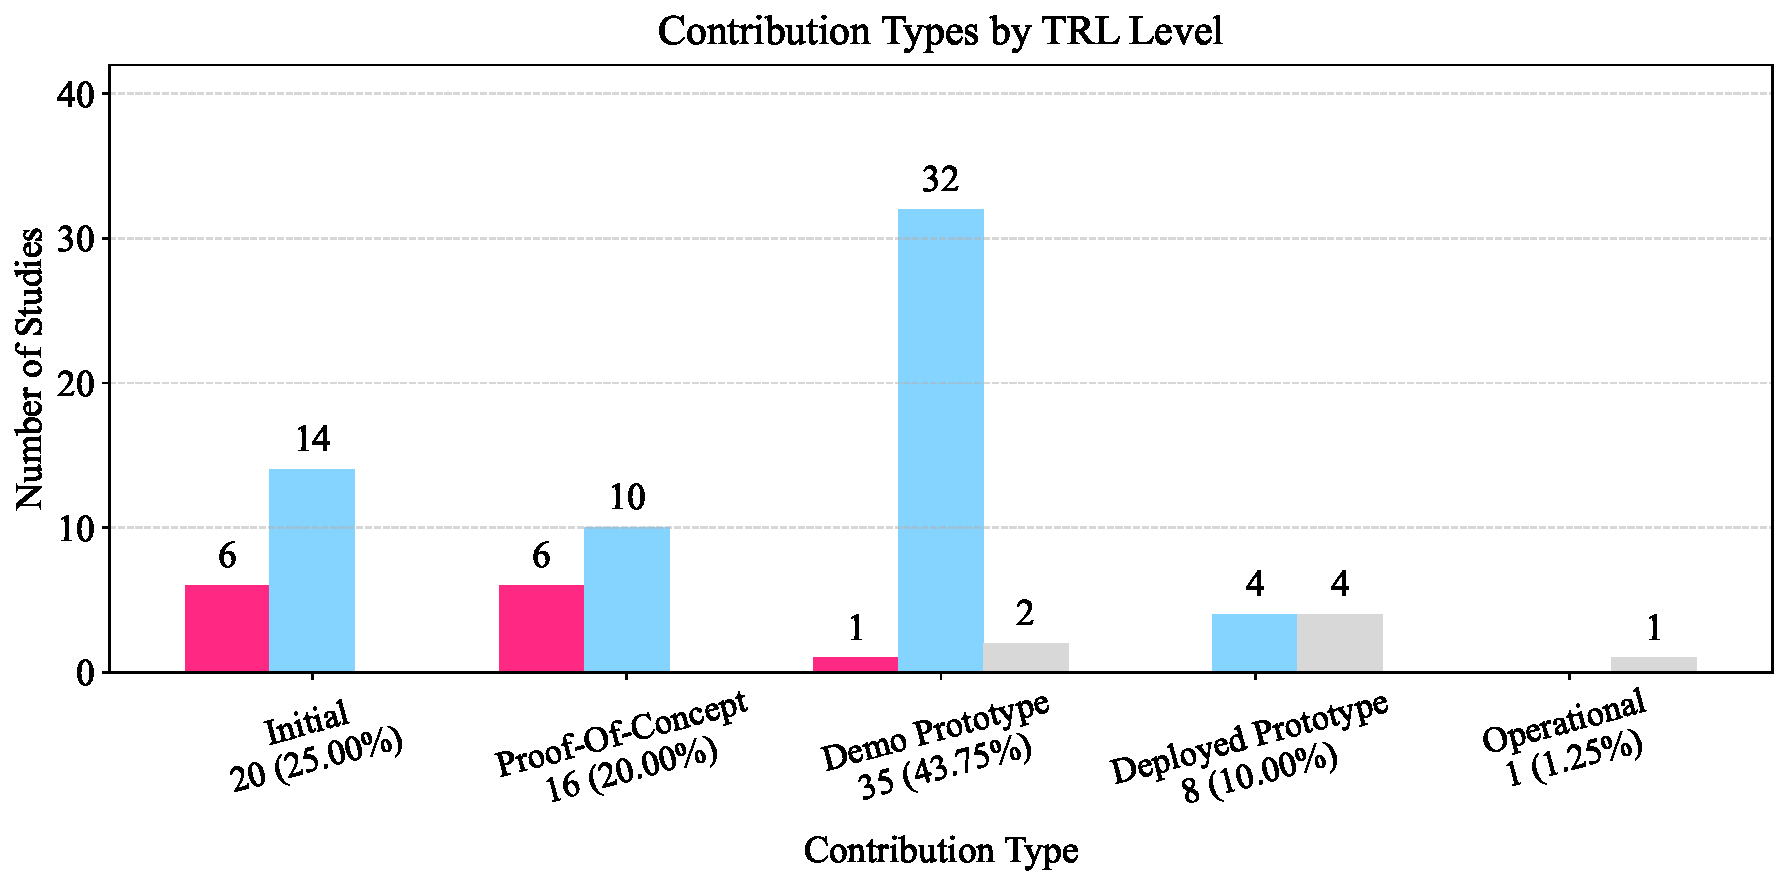
\includegraphics[width=0.9\linewidth]{figures/Literature Review/rq6/trlVsContributionType.pdf}
    \caption{Distribution of contribution types across TRLs}
    \caption*{{
    \color[HTML]{FF2882}\ding{110}} Conceptual
    ~~~{\color[HTML]{85d4ff}\ding{110}} Technical
    ~~~{\color[HTML]{d8d8d8}\ding{110}} Case Study
    }
    \label{fig:trl-v-cont}
\end{figure*}

\tabref{tab:trl-table} shows that most studies operate at lower-to-mid maturity, with demonstrative prototypes being the most common stage (\xofyp{35}{80}), followed by initial (\xofyp{20}{80}) and proof-of-concept efforts (\xofyp{16}{80}). Only a few studies report deployed prototypes (\xofyp{8}{80}) or fully operational systems (\xofyp{1}{80}).

\begin{table*}[htp]
\centering
\setlength{\tabcolsep}{1em}
\caption{Validation and evaluation approaches}
\label{tab:evaluation-structured-table}
\scriptsize
\begin{tabular}{@{}p{5cm} l p{7cm}@{}}
\toprule
\textbf{Evaluation Category} & \textbf{Frequency} & \textbf{Studies} \\
\midrule
\textbf{Validation} & \textbf{\maindatabar{72}} & \\
\;\;\corner{} Prototyping & \subdatabar{36} & \cite{aziz2022empowering,bao2024digital,bellavista2023requirements,chavezbaliguat2023digital,dahmen2022modeling,doubell2023digital,duan2023digital,ehemann2023digital,gil2023modeling,gollner2022collaborative,heininger2021capturing,heithoff2023challenges,hofmeister2024semantic,howard2021greenhouse,jiang2022novel,jirsa2024use,larsen2024towards,li2022cognitive,li2024comprehensive,liu2020web-based,lopez2023modeling,marah2023architecture,monsalve2021novel,novak2022digitalized,oquendo2019dealing,park2020digital,parri2019jarvis,parri2021framework,pickering2023towards,reiche2021digital,samak2023autodrive,saraeian2022digital,somma2023digital,stary2022privacy,villalonga2021decision-making,wagner2023using} \\
\;\;\corner{} Empirical Simulation & \subdatabar{16} & \cite{barden2022academic,chen2018digital,clark2021chapter,demir2023vertically-integrated,dickopf2019holistic,hatledal2020co-simulation,hofmeister2024cross-domain,kulkarni2019towards,lee2022simulation,lippi2023enabling,maheshwari2022digital,pillai2023digital,potteiger2023live,schluse2017experimentable,vogel-heuser2021approach,zhang2021bi-level} \\
\;\;\corner{} Architectural/Conceptual Design & \subdatabar{13} & \cite{altamiranda2019system,becue2018cyberfactory,dobie2024network,esterle2021digital,folds2019digital,hatakeyama2018systems,human2023design,joseph2021aggregated,kruger2022towards,redelinghuys2020six-layer,vermesan2021internet,wang2024construction,wullink2024foundational} \\
\;\;\corner{} Laboratory Experiments & \subdatabar{4} & \cite{acharya2023twins,gil2024integrating,priyanta2024is,savur2019hrc-sos} \\
\;\;\corner{} Mathematical Analysis & \subdatabar{3} & \cite{alam2017c2ps,kutzke2021subsystem,mahoro2023articulating} \\
\textbf{Evaluation} & \textbf{\maindatabar{8}} & \\
\;\;\corner{} Industrial Case Study & \subdatabar{7} & \cite{ashtaritalkhestani2019architecture,binder2021utilizing,coupaye2023graph-based,gill2022method,malayjerdi2022combined,mavromatis2024umbrella,zhang2022multi-scale} \\
\;\;\corner{} Action Research & \subdatabar{1} & \cite{bertoni2022digital} \\
\bottomrule
\end{tabular}
\end{table*}


In terms of contribution types (\tabref{tab:contribution-type-table}), the vast majority are technical contributions (\xofyp{60}{80}), often proposing new architectures or implementations. Conceptual works (\xofyp{13}{80}) make up a smaller portion of the sample, and case studies are underrepresented (\xofyp{7}{80}).

As illustrated in \figref{fig:trl-v-cont}, technical contributions are the most typical across all TRLs but especially in demo prototypes and initial stages. Conceptual works appear mostly at lower TRLs. Case studies, i.e., in-depth investigations of a real-world, contemporary phenomena within their actual contexts~\cite{crowe2011case}, are rarely found and only emerge beyond the initial and proof-of-concept stages. This reflects a strong emphasis on engineering feasibility but limited real-world validation.

\subsubsection{Evaluation}\label{sec:evaluation}

\tabref{tab:evaluation-structured-table} shows that validation research (\xofyp{72}{80}) dominates the sample, mainly through prototyping (\xofyp{36}{80}), simulation (\xofyp{16}{80}), and conceptual design validation (\xofyp{13}{80}). Along with laboratory experiments (\xofyp{4}{80}) and mathematical analysis (\xofyp{3}{80}). For example, \textcite{hatledal2020co-simulation} and \textcite{chen2018digital} use simulation to validate co-simulated and behavior-predictive DTs, respectively. \textcite{larsen2024towards} prototype a DTaaS platform for robot composition, while \textcite{redelinghuys2020six-layer} validate architecture designs through structured frameworks and applied case studies. Mathematical analysis is used in \textcite{mahoro2023articulating} to formalize graph-based synchronization across DT layers. \textcite{savur2019hrc-sos} conduct laboratory experiments to evaluate a human-robot collaboration system through physical trials.

In contrast, evaluation research appears in only (\xofyp{8}{80}) studies. \textcite{ashtaritalkhestani2019architecture} conduct an industrial case study to assess DT-based automation, and \textcite{bertoni2022digital} apply action research to support planning in mining operations using an operational DT.



\subsubsection{Standards}\label{sec:standards}

\begin{table*}[]
            \centering
            \footnotesize
            \caption{Standards}
            \label{tab:standards-table}
            \begin{tabular}{@{}p{4cm}l p{8.5cm}@{}}
            \toprule
            \multicolumn{1}{c}{\textbf{Standard}} & 
            \multicolumn{1}{c}{\textbf{Frequency}} & 
            \multicolumn{1}{c}{\textbf{Studies}} \\ 
            \midrule
            Open Platform Communications Unified Architecture (OPC UA) & \maindatabar{13} & \cite{acharya2023twins,ashtaritalkhestani2019architecture,binder2021utilizing,dobie2024network,gollner2022collaborative,howard2021greenhouse,jirsa2024use,joseph2021aggregated,liu2020web-based,novak2022digitalized,redelinghuys2020six-layer,reiche2021digital,villalonga2021decision-making} \\
IEC 63278: Asset Administration Shell & \maindatabar{8} & \cite{acharya2023twins,ashtaritalkhestani2019architecture,gil2023modeling,gill2022method,gollner2022collaborative,jirsa2024use,reiche2021digital,vogel-heuser2021approach} \\
Reference Architectural Model Industrie 4.0 (RAMI 4.0) & \maindatabar{4} & \cite{binder2021utilizing,gill2022method,human2023design,park2020digital} \\
Other & \maindatabar{26} & \cite{alam2017c2ps,altamiranda2019system,ashtaritalkhestani2019architecture,barden2022academic,bellavista2023requirements,binder2021utilizing,dickopf2019holistic,dobie2024network,gollner2022collaborative,hatledal2020co-simulation,heininger2021capturing,heithoff2023challenges,howard2021greenhouse,human2023design,jiang2022novel,li2022cognitive,malayjerdi2022combined,monsalve2021novel,novak2022digitalized,parri2019jarvis,parri2021framework,pickering2023towards,savur2019hrc-sos,stary2022privacy,vermesan2021internet,vogel-heuser2021approach} \\
\bottomrule
            \end{tabular}
            \end{table*}
\begin{table*}[htp]
            \centering
            \scriptsize
            \caption{Standards usage context (DT vs. SoS)}
            \label{tab:dt-or-sos-related-table}
            \begin{tabular}{@{}p{4cm}l p{8.5cm}@{}}
            \toprule
            \multicolumn{1}{c}{\textbf{Context}} & 
            \multicolumn{1}{c}{\textbf{Frequency}} & 
            \multicolumn{1}{c}{\textbf{Studies}} \\ 
            \midrule
            DT & \maindatabar{18} & \cite{acharya2023twins,alam2017c2ps,bellavista2023requirements,binder2021utilizing,dickopf2019holistic,gil2023modeling,gill2022method,gollner2022collaborative,hatledal2020co-simulation,heininger2021capturing,heithoff2023challenges,jirsa2024use,joseph2021aggregated,liu2020web-based,malayjerdi2022combined,reiche2021digital,stary2022privacy,villalonga2021decision-making} \\
SoS & \maindatabar{10} & \cite{altamiranda2019system,barden2022academic,howard2021greenhouse,li2022cognitive,monsalve2021novel,park2020digital,pickering2023towards,redelinghuys2020six-layer,savur2019hrc-sos,vermesan2021internet} \\
Both & \maindatabar{6} & \cite{ashtaritalkhestani2019architecture,dobie2024network,human2023design,jiang2022novel,novak2022digitalized,vogel-heuser2021approach} \\
\bottomrule
            \end{tabular}
            \end{table*}
\begin{table*}[]
\centering
\setlength{\tabcolsep}{1em}
\caption{Programming languages and data formats}
\label{tab:programming-languages-structured-table}
\scriptsize
\begin{tabular}{@{}p{5cm} l p{7.5cm}@{}}
\toprule
\textbf{Category} & \textbf{Frequency} & \textbf{Studies} \\
\midrule
\textbf{General Purpose} & \textbf{\maindatabar{36}} & \\
\;\;\corner{} Python & \subdatabar{22} & \cite{bao2024digital,barden2022academic,bellavista2023requirements,chavezbaliguat2023digital,doubell2023digital,duan2023digital,gil2023modeling,jirsa2024use,lippi2023enabling,liu2020web-based,maheshwari2022digital,malayjerdi2022combined,marah2023architecture,mavromatis2024umbrella,monsalve2021novel,park2020digital,potteiger2023live,samak2023autodrive,saraeian2022digital,savur2019hrc-sos,vogel-heuser2021approach,wagner2023using} \\
\;\;\corner{} Java & \subdatabar{14} & \cite{alam2017c2ps,ashtaritalkhestani2019architecture,aziz2022empowering,bellavista2023requirements,clark2021chapter,gil2023modeling,gil2024integrating,hatledal2020co-simulation,li2024comprehensive,marah2023architecture,parri2019jarvis,parri2021framework,vogel-heuser2021approach,wagner2023using} \\
\;\;\corner{} JavaScript & \subdatabar{8} & \cite{bao2024digital,barden2022academic,doubell2023digital,duan2023digital,hofmeister2024semantic,liu2020web-based,priyanta2024is,samak2023autodrive} \\
\;\;\corner{} C++ & \subdatabar{4} & \cite{hatledal2020co-simulation,mavromatis2024umbrella,park2020digital,samak2023autodrive} \\
\;\;\corner{} C\# & \subdatabar{3} & \cite{lee2022simulation,park2020digital,redelinghuys2020six-layer} \\
\;\;\corner{} C & \subdatabar{1} & \cite{hatledal2020co-simulation} \\
\;\;\corner{} Xtend & \subdatabar{1} & \cite{oquendo2019dealing} \\
\;\;\corner{} Jython & \subdatabar{1} & \cite{wagner2023using} \\
\textbf{Data Representation} & \textbf{\maindatabar{12}} & \\
\;\;\corner{} XML & \subdatabar{9} & \cite{ashtaritalkhestani2019architecture,binder2021utilizing,dahmen2022modeling,jiang2022novel,jirsa2024use,kutzke2021subsystem,monsalve2021novel,oquendo2019dealing,redelinghuys2020six-layer} \\
\;\;\corner{} JSON & \subdatabar{5} & \cite{acharya2023twins,aziz2022empowering,dahmen2022modeling,jirsa2024use,vogel-heuser2021approach} \\
\textbf{Markup and Styling} & \textbf{\maindatabar{4}} & \\
\;\;\corner{} HTML & \subdatabar{4} & \cite{bao2024digital,doubell2023digital,hofmeister2024semantic,samak2023autodrive} \\
\;\;\corner{} CSS & \subdatabar{4} & \cite{bao2024digital,doubell2023digital,hofmeister2024semantic,samak2023autodrive} \\
\bottomrule
\end{tabular}
\end{table*}

\tabref{tab:standards-table} summarizes standards referenced across the studies. Open Platform Communications Unified Architecture (OPC UA) is the most used (\xofyp{13}{80}), supporting secure communication and hierarchical data exchange \cite{dobie2024network, joseph2021aggregated}. IEC 63278 (Asset Administration Shell) appears in (\xofyp{8}{80}) studies for asset representation and interoperability \cite{gill2022method, gollner2022collaborative}. Reference Architectural Model Industrie 4.0 (RAMI 4.0) is cited in (\xofyp{4}{80}) studies to guide structured DT integration \cite{binder2021utilizing}. Other domain-specific standards include VANET, IPv6 \cite{alam2017c2ps}, ISO/IEC/IEEE 15288 \cite{altamiranda2019system}, ISA-95 \cite{dobie2024network}, IEC 61850 \cite{jiang2022novel}, and IEEE 1451 \cite{li2022cognitive}. Security-related standards include GDPR \cite{stary2022privacy} and OAuth 2.0 \cite{human2023design, jiang2022novel}.

\begin{table*}[]
\centering
\setlength{\tabcolsep}{1em}
\caption{Tools and frameworks}
\label{tab:frameworks-structured-table}
\scriptsize
\begin{tabular}{@{}p{5cm} l p{7.5cm}@{}}
\toprule
\textbf{Category} & \textbf{Frequency} & \textbf{Studies} \\
\midrule
\textbf{Modeling \& Simulation} & \textbf{\maindatabar{35}} & \\
\;\;\corner{} MATLAB & \subdatabar{10} & \cite{ashtaritalkhestani2019architecture,bertoni2022digital,chen2018digital,kutzke2021subsystem,larsen2024towards,lopez2023modeling,novak2022digitalized,reiche2021digital,schluse2017experimentable,zhang2022multi-scale} \\
\;\;\corner{} Simulink & \subdatabar{4} & \cite{ashtaritalkhestani2019architecture,lopez2023modeling,novak2022digitalized,zhang2022multi-scale} \\
\;\;\corner{} Modelica & \subdatabar{4} & \cite{ashtaritalkhestani2019architecture,howard2021greenhouse,larsen2024towards,zhang2022multi-scale} \\
\;\;\corner{} Gazebo & \subdatabar{4} & \cite{esterle2021digital,mavromatis2024umbrella,savur2019hrc-sos,schluse2017experimentable} \\
\;\;\corner{} Tecnomatix & \subdatabar{3} & \cite{gill2022method,redelinghuys2020six-layer,schluse2017experimentable} \\
\;\;\corner{} AnyLogic & \subdatabar{3} & \cite{howard2021greenhouse,joseph2021aggregated,marah2023architecture} \\
\;\;\corner{} CARLA Simulator & \subdatabar{2} & \cite{malayjerdi2022combined,potteiger2023live} \\
\;\;\corner{} Java Agent Development Framework (JADE) & \subdatabar{2} & \cite{marah2023architecture,vogel-heuser2021approach} \\
\;\;\corner{} Virtual Robotics Experimentation Platform (V-REP) & \subdatabar{2} & \cite{savur2019hrc-sos,schluse2017experimentable} \\
\;\;\corner{} \textit{Other} & \subdatabar{22} & \cite{acharya2023twins,alam2017c2ps,dahmen2022modeling,gil2023modeling,gollner2022collaborative,hatledal2020co-simulation,heithoff2023challenges,howard2021greenhouse,larsen2024towards,li2022cognitive,lopez2023modeling,marah2023architecture,monsalve2021novel,novak2022digitalized,oquendo2019dealing,park2020digital,parri2019jarvis,potteiger2023live,priyanta2024is,saraeian2022digital,savur2019hrc-sos,vogel-heuser2021approach} \\
\textbf{Data Management} & \textbf{\maindatabar{19}} & \\
\;\;\corner{} MongoDB & \subdatabar{6} & \cite{aziz2022empowering,dobie2024network,larsen2024towards,somma2023digital,villalonga2021decision-making,zhang2021bi-level} \\
\;\;\corner{} PostgreSQL & \subdatabar{3} & \cite{doubell2023digital,human2023design,mavromatis2024umbrella} \\
\;\;\corner{} InfluxDB & \subdatabar{3} & \cite{larsen2024towards,li2024comprehensive,mavromatis2024umbrella} \\
\;\;\corner{} Redis & \subdatabar{3} & \cite{li2024comprehensive,liu2020web-based,zhang2021bi-level} \\
\;\;\corner{} Prometheus & \subdatabar{2} & \cite{bellavista2023requirements,mavromatis2024umbrella} \\
\;\;\corner{} Protégé & \subdatabar{2} & \cite{gil2024integrating,liu2020web-based} \\
\;\;\corner{} MySQL & \subdatabar{2} & \cite{li2024comprehensive,liu2020web-based} \\
\;\;\corner{} \textit{Other} & \subdatabar{9} & \cite{chavezbaliguat2023digital,clark2021chapter,dahmen2022modeling,dobie2024network,hofmeister2024semantic,jirsa2024use,li2024comprehensive,pickering2023towards,zhang2021bi-level} \\
\textbf{Geospatial \& Visualization} & \textbf{\maindatabar{19}} & \\
\;\;\corner{} Unity & \subdatabar{5} & \cite{chen2018digital,esterle2021digital,gil2023modeling,samak2023autodrive,schluse2017experimentable} \\
\;\;\corner{} WebGL & \subdatabar{2} & \cite{duan2023digital,li2024comprehensive} \\
\;\;\corner{} Microsoft Kinect & \subdatabar{2} & \cite{joseph2021aggregated,savur2019hrc-sos} \\
\;\;\corner{} \textit{Other} & \subdatabar{14} & \cite{barden2022academic,bertoni2022digital,chavezbaliguat2023digital,coupaye2023graph-based,duan2023digital,hofmeister2024semantic,human2023design,joseph2021aggregated,li2024comprehensive,malayjerdi2022combined,mavromatis2024umbrella,pickering2023towards,savur2019hrc-sos,somma2023digital} \\
\textbf{Digital Twin \& IoT} & \textbf{\maindatabar{15}} & \\
\;\;\corner{} Eclipse Ditto & \subdatabar{4} & \cite{acharya2023twins,aziz2022empowering,larsen2024towards,marah2023architecture} \\
\;\;\corner{} Robot Operating System (ROS) & \subdatabar{4} & \cite{mavromatis2024umbrella,pickering2023towards,samak2023autodrive,savur2019hrc-sos} \\
\;\;\corner{} Eclipse Arrowhead & \subdatabar{2} & \cite{acharya2023twins,aziz2022empowering} \\
\;\;\corner{} FIWARE & \subdatabar{2} & \cite{coupaye2023graph-based,somma2023digital} \\
\;\;\corner{} Thing’in & \subdatabar{2} & \cite{coupaye2023graph-based,mahoro2023articulating} \\
\;\;\corner{} \textit{Other} & \subdatabar{6} & \cite{acharya2023twins,dickopf2019holistic,gil2023modeling,jirsa2024use,joseph2021aggregated,marah2023architecture} \\
\textbf{Systems Eng. \& Architecture} & \textbf{\maindatabar{11}} & \\
\;\;\corner{} Enterprise Architect & \subdatabar{2} & \cite{binder2021utilizing,kutzke2021subsystem} \\
\;\;\corner{} Cameo Systems Modeler & \subdatabar{2} & \cite{dickopf2019holistic,wagner2023using} \\
\;\;\corner{} Metasonic Suite & \subdatabar{2} & \cite{heininger2021capturing,stary2022privacy} \\
\;\;\corner{} \textit{Other} & \subdatabar{7} & \cite{dobie2024network,larsen2024towards,lopez2023modeling,mavromatis2024umbrella,pickering2023towards,stary2022privacy,wagner2023using} \\
\textbf{App/Web Technologies} & \textbf{\maindatabar{10}} & \\
\;\;\corner{} .NET Framework & \subdatabar{2} & \cite{lee2022simulation,park2020digital} \\
\;\;\corner{} \textit{Other} & \subdatabar{10} & \cite{aziz2022empowering,chavezbaliguat2023digital,doubell2023digital,duan2023digital,esterle2021digital,larsen2024towards,lee2022simulation,li2022cognitive,liu2020web-based,park2020digital} \\
\textbf{Cloud, Edge, and DevOps} & \textbf{\maindatabar{8}} & \\
\;\;\corner{} Docker & \subdatabar{5} & \cite{bellavista2023requirements,hofmeister2024semantic,mavromatis2024umbrella,monsalve2021novel,pickering2023towards} \\
\;\;\corner{} Kubernetes & \subdatabar{2} & \cite{bellavista2023requirements,mavromatis2024umbrella} \\
\;\;\corner{} Azure & \subdatabar{2} & \cite{larsen2024towards,pickering2023towards} \\
\;\;\corner{} \textit{Other} & \subdatabar{4} & \cite{bellavista2023requirements,demir2023vertically-integrated,mavromatis2024umbrella,redelinghuys2020six-layer} \\
\textbf{AI, Data Analytics \& ML} & \textbf{\maindatabar{7}} & \\
\;\;\corner{} Grafana & \subdatabar{3} & \cite{bellavista2023requirements,esterle2021digital,mavromatis2024umbrella} \\
\;\;\corner{} Jupyter Lab & \subdatabar{2} & \cite{chavezbaliguat2023digital,larsen2024towards} \\
\;\;\corner{} \textit{Other} & \subdatabar{3} & \cite{joseph2021aggregated,malayjerdi2022combined,mavromatis2024umbrella} \\
\bottomrule
\end{tabular}
\end{table*}


\tabref{tab:dt-or-sos-related-table} shows that most standards are applied in DT specific contexts (\xofyp{18}{80}), fewer relate to SoS (\xofyp{10}{80}), and only (\xofyp{6}{80}) support both. DT-oriented examples include the use of OPC UA and RAMI 4.0 for modeling and communication \cite{binder2021utilizing}. SoS-focused rely on NATO and SISO standards to support coordination and mission-level system integration\cite{barden2022academic}. \textcite{vermesan2021internet} present a combined view, applying both DT and SoS-relevant standards in the Internet of Vehicles (IoV) context.
In total, \xofy{36}{80}{} unique studies rely on a standard, i.e., the majority of the sampled studies does not adhere to standards.



\begin{conclusionframe}{RQ6: Maturity of SoTS research}
SoTS research in our sample, even after rigorous quality criteria, is situated largely at low-to-mid TRLs, with demo prototypes and proof-of-concept efforts being the most common.
Validation is primarily conducted through prototyping and simulation, with limited empirical evaluation. Standards are inconsistently applied and tend to focus on DT-specific components, with few addressing SoS integration or supporting both layers.
\end{conclusionframe}


\subsection{What technology is used to implement systems that combine SoS and DT? (RQ7)}\label{results-rq7}

To understand what technologies support the implementation of SoTS, we examine the programming languages and data formats used (\secref{sec:programming-languages}), as well as the development frameworks and platforms adopted across studies (\secref{sec:frameworks}).



\subsubsection{Programming languages and formats}\label{sec:programming-languages}

\tabref{tab:programming-languages-structured-table} shows that most studies rely on general-purpose programming languages (\xofyp{36}{80}), particularly Python (\xofyp{22}{80}) and Java (\xofyp{14}{80}), reflecting their flexibility in data processing and simulation. Languages like JavaScript, C++, and C\# appear less frequently.
Data representation formats are used in (\xofyp{12}{80}) studies, with XML (\xofyp{9}{80}) and JSON (\xofyp{5}{80}) supporting structured data exchange.
Markup and styling languages, e.g., HTML and CSS, appear in (\xofyp{4}{80}) cases each, usually for visualization or web-based system interfaces.



\subsubsection{Frameworks and platforms}\label{sec:frameworks}


\tabref{tab:frameworks-structured-table} shows that most studies use modeling and simulation tools (\xofyp{35}{80}), notably MATLAB (\xofyp{10}{80}), Gazebo, Modelica, and Simulink (each \xofyp{4}{80}), supporting system dynamics and co-simulation.
Data management tools appear in (\xofyp{19}{80}) studies, with MongoDB (\xofyp{6}{80}) leading. Other tools like PostgreSQL, Redis, and Protégé support storage, synchronization, and ontology modeling.
Visualization tools are also common (\xofyp{19}{80}), with Unity (\xofyp{5}{80}) and platforms like WebGL and Kinect enabling interactive 3D or AR interfaces.
DT and IoT platforms are used in (\xofyp{15}{80}), including Eclipse Ditto and ROS (each \xofyp{4}{80}) supporting twin orchestration, and device interoperability.
Systems engineering tools (\xofyp{11}{80}), like Cameo Systems Modeler, Metasonic Suite, and Enterprise Architect, support architectural modeling.
Other categories include web/app frameworks (\xofyp{10}{80}), cloud and DevOps tools (\xofyp{8}{80}) like Docker and Azure, and analytics platforms (\xofyp{7}{80}), e.g., Grafana and Jupyter Lab for monitoring and machine learning (ML).

\begin{conclusionframe}{RQ7: Technologies used in SoTS}
Systems combining SoS and DT use diverse technologies, with Python and Java as primary languages and XML/JSON for data formatting. The frameworks used focus on supporting simulation, data management, and systems engineering.
\end{conclusionframe}